\documentclass[12pt]{article}
% adjust style for page
\usepackage{fancyhdr}
% adjust the gap between content and margins of pages 
\usepackage{geometry}
% import images
\usepackage{graphicx} 
% tweak math elements
\usepackage{amsmath}
% import other .tex files into the main .tex
\usepackage{import}
% for simulating model content
\usepackage{lipsum}
% for hyper link that connects to other URL
\usepackage{hyperref}
% for tables having specific width
\usepackage{tabularx} 
% together used with "tabularx" package
\usepackage{booktabs}
% control position of elements precisely
\usepackage{float}
% control the caption element for table and figure
\usepackage{caption}
% for some math symbols and format
\usepackage{amsmath} % for 'cases' environment
% To manage footnotes in tables
\usepackage{threeparttable}  
% i forget the function of this one, GPT told me to include it :) 
\usepackage{babel}
% for multirows
\usepackage{multirow}
% for biblatex
% \usepackage[backend=biber]{biblatex}
% for hyper link
\usepackage{hyperref}

\newenvironment{myfigure}[3] % width, path, caption
{
    \begin{figure}[htbp]
        \centering
        \includegraphics[width=#1\textwidth]{#2}
        \caption{#3}
}
{
    \end{figure}
}
\usepackage{xcolor}
\usepackage{array}
\usepackage[skip=2pt, labelfont=it, textfont=it, font=small]
{caption}
\usepackage{subcaption}
\usepackage{graphicx} 
\usepackage{amsmath}    % For advanced math formatting
\usepackage{amssymb}    % For additional math symbols
\usepackage{amsfonts}   % For math fonts like \mathbb



\definecolor{myyellow}{RGB}{255, 255, 150}

\newcolumntype{M}[1]{>{\centering\arraybackslash}m{#1}}

\title{
This is title
}

\author{Feng Gu(T00751197), author 2 and author 3}

\begin{document}
\maketitle

\begin{center}
    \textbf{\large Abstract}
    Here to attach abstract.
\end{center}

% \begin{frame}
    \frametitle{Introduction}
    \begin{itemize}
        \item Brief overview of the project
        \item Objectives and goals
        \item Importance of the topic
    \end{itemize}
\end{frame}
% \section{Data Description and EDA}


We summarized the dataset's key statistics to identify trends, central tendencies, and potential anomalies in the data.
Descriptive summaries provided insights into the distribution of 
demographic, clinical, and hospitalization-related variables.

\textcolor{red}{table and figures in appendix}

Many of the numerical variables exhibited significant skewness and the presence of outliers.

\begin{itemize}
    \item \textbf{Shapiro-Wilk Test:} This test confirmed that nearly all variables deviated significantly from normality.
    \item \textbf{Skewness and Kurtosis:} These measures indicated that several variables had heavy-tailed distributions. This finding suggested the need for scaling and normalization techniques to ensure reliable modeling.
\end{itemize}

To explore inter-variable relationships and assess the risk of multicollinearity,
 we performed a correlation analysis across the dataset. 
The results(Figure \ref{fig:correlation_matrix}) identified strong linear relationships among several variable groups:

\begin{figure}[!h]
    \centering
    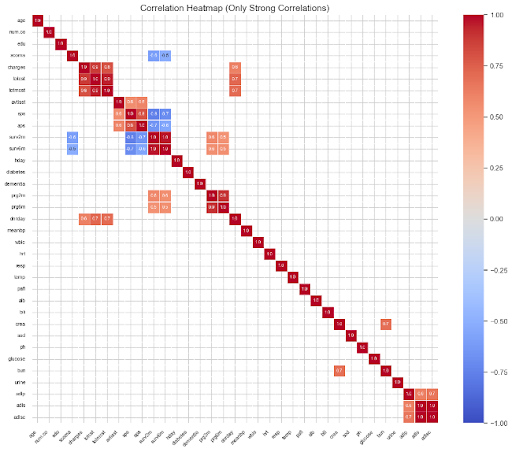
\includegraphics[width=0.8\textwidth]{../results/correlation_target.png}
    \caption{Correlation matrix of the SUPPORT2 dataset.}
    \label{fig:correlation_matrix}
\end{figure}

\begin{itemize}
    \item \textbf{Medical Cost Variables:} \texttt{charges}, \texttt{totcst}, and \texttt{totmcst} showed high positive correlations.
    \item \textbf{Physiological Measures:} \texttt{aps}, \texttt{sps}, and \texttt{avtisst} demonstrated strong internal correlations.
    \item \textbf{Survival Probabilities:} \texttt{surv2m}, \texttt{surv6m}, \texttt{prg2m}, and \texttt{prg6m} were highly correlated, suggesting they reflect overlapping prognostic information.
    \item \textbf{Activities of Daily Living (ADL):} \texttt{adlp}, \texttt{adls}, and \texttt{adlsc} were also strongly related.
\end{itemize}

Understanding the distribution of our target variable \texttt{sfdm2} is crucial for selecting appropriate modeling approaches and evaluation metrics. SFDM2 quantifies patient functional disability on a 1--5 severity scale, with 5 representing maximum impairment. This metric was derived from Sickness 
Impact Profile (SIP) questionnaires via patients and/or their surrogates to systematically evaluate functional status.

\begin{table}[H]
    \centering
    \renewcommand{\arraystretch}{1.5} % Optional: adds vertical padding
    \caption{SFDMS Category Descriptions}
    \begin{tabular}{|M{1.5cm}|M{4cm}|M{7cm}|}
    \hline
    \textbf{Level} & \textbf{Class Name} & \textbf{Meanings} \\
    \hline
    1 & no (Month 2 \& SIP present) & No signs of moderate to severe functional disability. \\
    \hline
    2 & adl $\geq$ 4 ($\geq$ 5 if survived) & Patient was unable to do 4 or more activities of daily living. \\
    \hline
    3 & SIP $\geq$ 30 & Sickness Impact Profile total score at 2 months is greater or equal to 30. \\
    \hline
    4 & Coma or Intubated & Patient intubated or in coma. \\
    \hline
    5 & $<$ 2 mo. follow-up & Patient died before 2 months after study entry. \\
    \hline
    \end{tabular}
\end{table}

The proportion of 5 different target values in response variable is shown in Figure\ref{fig:train_test_target_proportion}.
This imbalance necessitates careful consideration during model development, 
potentially requiring techniques such as resampling,class weighting, or specialized algorithms.

\textcolor{red}{figure in appendix}
% \section{Data Preprocessing and feature selection}

\subsection{Missing Value Imputation}

The dataset contains 9105 rows and 48 columns with varying degrees of missingness(Figure \ref{fig:missing_distribution}).:

\begin{itemize}
    \item \textbf{Target Variable (\texttt{sfdm2}):} Missing in 1400 rows (15.38\%). These rows were removed to avoid data leakage, as imputing the target variable would undermine model integrity.
    \item \textbf{Predictor Variables:} 32 variables had missing values, with some exceeding 50\% (e.g., \texttt{adlp}, \texttt{urine}).
\end{itemize}

\begin{figure}[!h]
\centering
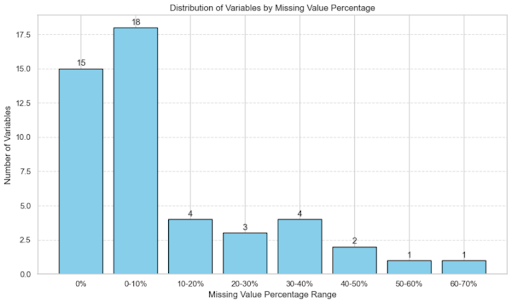
\includegraphics[width=0.8\textwidth]{../results/missing_distribution.png}
\caption{Distribution of missing values in the dataset}
\label{fig:missing_distribution}
\end{figure}

To address missing values, we employed a combination of clinical imputation and custom imputation pipelines. 
The imputation process was designed to ensure that the data remained representative and suitable for modeling.

\begin{enumerate}
    \item \textbf{Clinical Imputation:} We used reference values from the dataset documentation to impute 7 clinical variables:
    \begin{itemize}
        \item \texttt{alb}: 3.5, \texttt{pafi}: 333.3, \texttt{bili}: 1.01, \texttt{crea}: 1.01, \texttt{bun}: 6.51, \texttt{wblc}: 9.0, \texttt{urine}: 2502
    \end{itemize}
    
    \item \textbf{Custom Imputation Pipelines:} We designed three imputer types tailored to the data types:
    \begin{table}[H]
    \centering
    \caption{Imputation Strategy Table}
    \begin{tabular}{|c|c|c|}
    \hline
    \textbf{Imputer Type} & \textbf{Variable Feature} & \textbf{Imputation Methods} \\
    \hline
    I   & Numerical        & Mean, Median, Constant, KNN \\
    II  & Categorical      & One-hot: Most frequent, Constant \texttt{Unknown} \\
    III & Categorical      & Simple: Most frequent, Constant \texttt{Unknown} \\
    \hline
    \end{tabular}
    \end{table}
\end{enumerate}

By combining the methods in each imputer type, we generated 16 distinct
imputed datasets (4 $\times$ 2 $\times$ 2) to enable comparative modeling.


\begin{figure}[!h]
\centering
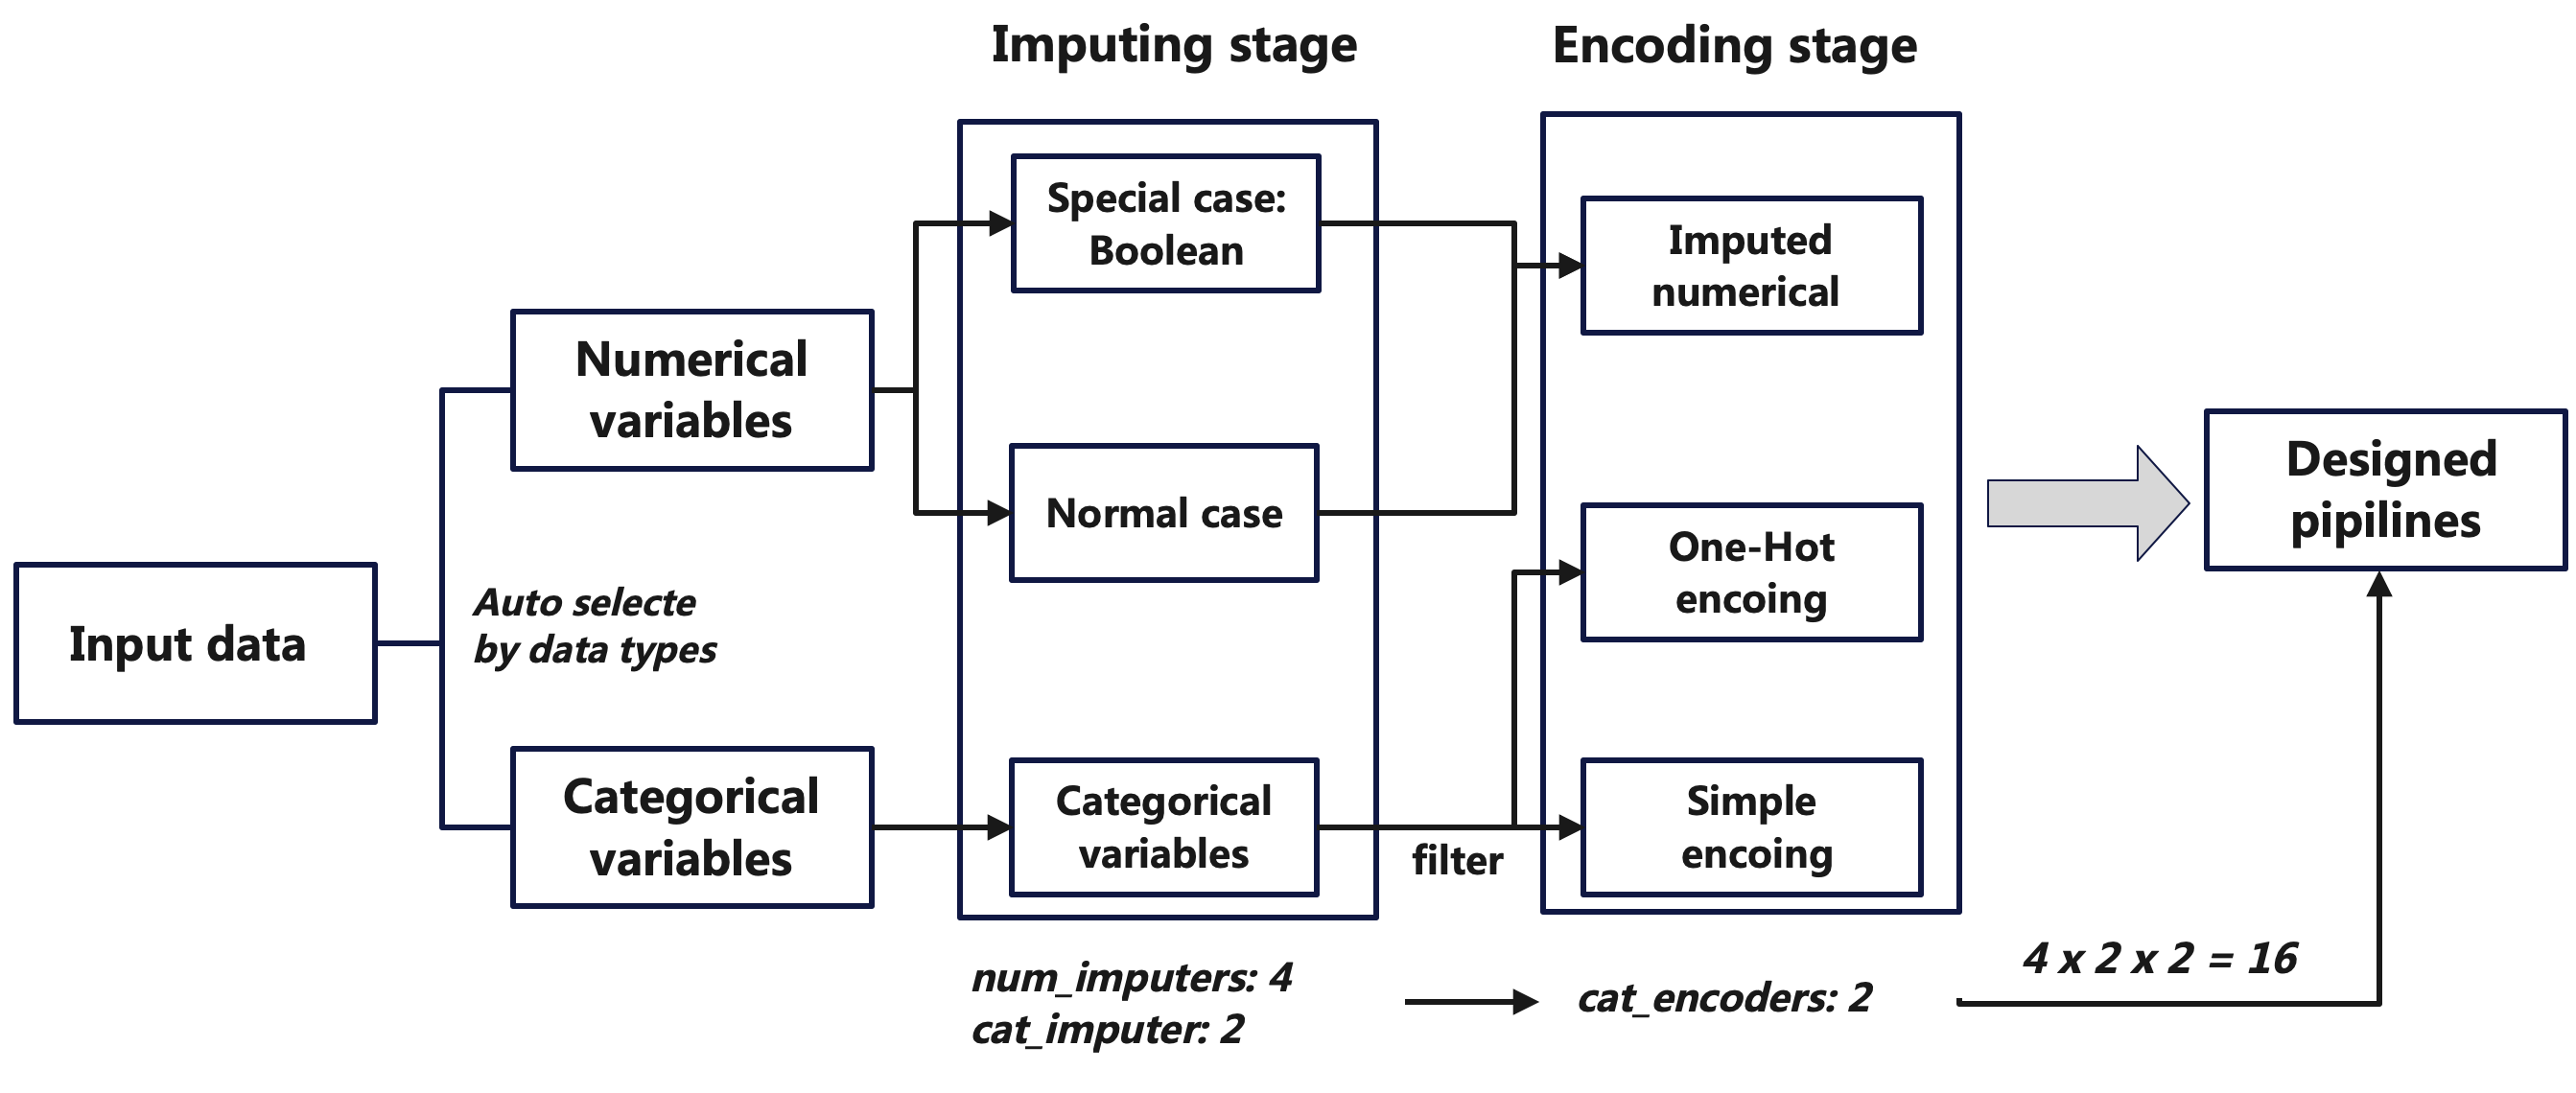
\includegraphics[width=0.8\textwidth]{../results/pipeline_imputing.png}
\caption{Design of Imputation Pipelines}
\label{fig:imputation_pipeline}
\end{figure}

\textbf{Simple Encoding:} For certain qualitative variables, 
simple imputation methods are not directly applicable due to their ordinal nature and
the arbitrary encoding generated by default functions. 
To address this, we established a custom mapping scheme for these variables,
as detailed in Table \ref{tab:encoding_mapping}.


\begin{table}[H]
    \centering
    \caption{Simple Encoding Mapping('--' indicates no mapping)}
    \label{tab:encoding_mapping}
    \begin{tabular}{|c|c|c|c|}
    \hline
    \textbf{Encoded} & \textbf{Income} & \textbf{DNR} & \textbf{SFDMS (sfdm2)} \\
    \hline
    0 & Unknown & Unknown & -- \\
    1 & Under \$11k & No DNR & No (Month 2 and SIP present) \\
    2 & \$11k-\$25k & DNR after SADM & ADL $\geq$ 4 (5 if survived) \\
    3 & \$25k-\$50k & DNR before SADM & SIP $\geq$ 30 \\
    4 & \>\$50k & -- & Coma or Intub \\
    5 & -- & -- & $<$ 2 mo. follow-up \\
    \hline
    \end{tabular}
\end{table}

\textbf{One-Hot Encoding:} Applied to multi-class categorical variables where 
the order of categories is not meaningful,
such as \texttt{sex}, \texttt{dzgroup}, and \texttt{dzclass}.


\subsection{Data Leakage Mitigation}

To ensure model generalizability, we removed variables that could leak information about the outcome:

\begin{itemize}
    \item \texttt{death}, \texttt{hospdead}, \texttt{slos}, \texttt{d.time} — these variables represent outcomes or timing after the 2-month period and can leak post-prediction information into training.
    \item Inclusion of these variables may indirectly reveal mortality and discharge timing, violating the principle that only pre-outcome data be used for prediction.
\end{itemize}

\subsection{Stratified Train-Test Split}

We performed an 80/20 split of the dataset, using stratified sampling to preserve the distribution of the \texttt{sfdm2} outcome variable.
Standardization was applied to all features to reduce outlier influence and ensure consistent data scale.

\textcolor{red}{fig in appendix}

\section{Feature Selection}

\section{Multiple Logistic Regression}

We applied MLR to each of selected sub datasets to identify the most accurate imputation strategy. The model predicts:
\[
P(Y = 1 \mid X) = \frac{e^{\beta_0 + \sum_{j=1}^{p} \beta_j X_j}}{1 + e^{\beta_0 + \sum_{j=1}^{p} \beta_j X_j}}
\]
where \( \beta_j \) are the coefficients estimated through log-likelihood maximization.

\subsection{LASSO Regularization}

We used Lasso regression to select the most important features from the dataset, and use the selected features to build the model.
The optimization problem for Lasso regression can be formulated as:

\[
\hat{\beta} = \arg\min_{\beta} \left\{ \frac{1}{n} \sum_{i=1}^n \left( y_i - \mathbf{x}_i^\top \beta \right)^2 + \lambda \sum_{j=1}^p |\beta_j| \right\}
\]

The reason we chose lasso instead of ridge is that the lasso penalty, \( \lambda \sum_{j=1}^p |\beta_j| \), encourages sparsity in the coefficients, 
which drop some of coefficients to zero when some features are highly correlated(shown in Figure \ref{fig:correlation_matrix}). However, ridge regression will not 
drop the highly correlated features, but will give them similar coefficients, which does not help to reduce the model complexity.

We tuned $\lambda$ using a stratified 5-fold cross-validation over a log-transformed range: $\log(1/\lambda)$ from $[-4, 2]$.

\subsection{Choosing of selected features and best imputation strategy}

We evaluated model performance across the 16 imputation pipelines:
\begin{itemize}
    \item \textbf{Best Imputation Strategy:} Imputer-2 achieved the highest accuracy of \textbf{71.87\%}.
    \item \textbf{Optimal} \( \lambda = 0.033598 \), selected using 5-fold cross-validation.
\end{itemize}

The final LASSO model retained 23 predictors, balancing interpretability with predictive strength.

For model simplicity, we selected the 14 most important predictors based 
on their significance in the LASSO regression result and their contribution to predicting \texttt{sfdm2}.

\begin{figure}[!h]
\centering
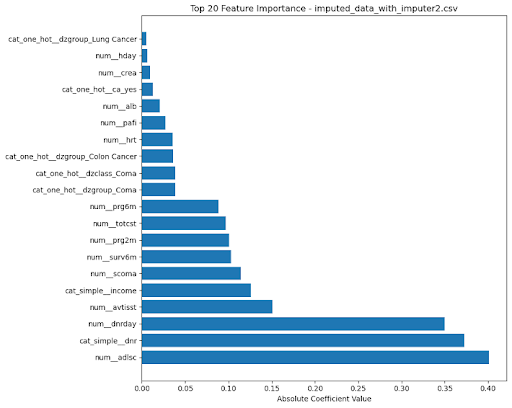
\includegraphics[width=0.8\textwidth]{../results/feature_selected_Lasso.png}
\caption{Rank of feature importantce in LASSO model}
\label{fig:feature_importance}
\end{figure}
% \section{Feature engineering for handling class imbalance}


Class imbalance in classification tasks can be addressed partially through feature engineering
techniques that modify the dataset to improve model performance on minority classes. 
Below, we explore three methods: Random Oversampling, SMOTE, and Augmented SMOTE.

\begin{itemize}
    \item \textbf{Random Oversampling:} 
    
    Random Oversampling duplicates minority class samples to balance class sizes with the majority class.
     While this method is computationally efficient, it may lead to overfitting due to repeated samples.

    \item \textbf{Synthetic Minority Oversampling Technique (SMOTE):} 
    
    SMOTE generates synthetic samples for minority 
    classes by interpolating between existing samples and their nearest neighbors.
    This approach ensures a more diverse dataset and reduces overfitting compared to simple oversampling.

    \item \textbf{Augmented SMOTE with PCA:} 
    
    Augmented SMOTE combines SMOTE with dimensionality reduction techniques like PCA to avoid over-synthesis in high-dimensional spaces. 
    By reducing the data to a lower-dimensional representation before applying SMOTE. 
    
    This method ensures meaningful interpolation and avoids overfitting. 
    Additionally, random undersampling of majority classes can be applied to further balance the dataset.
\end{itemize}

\subsection{Class Imbalance Mitigation}

From the exploratory data analysis (EDA), it became evident that the target variable (sfdm2) exhibits a pronounced class imbalance. 
The majority of observations belong to Class 1 and Class 5, while Class 4 accounts for less than 0.5\% of the total data. 
Such a skewed distribution can significantly hinder a model's ability to learn meaningful patterns associated with minority classes, 
often resulting in poor generaliza-tion on these underrepresented groups. To evaluate the impact of this imbalance, we trained a baseline
Random Forest model using the original (imbalanced) training data without applying any resampling or class weighting strategies, 
and then assessed its performance on the test set.
The results of this baseline model are summarized below


\begin{table}[!h]
\centering
\caption{Classification Report (upon original Imbalanced Data)}
\label{tab:rf_imbalanced}
\begin{tabular}{|c|c|c|c|c|}
\hline
\textbf{Class} & \textbf{Precision} & \textbf{Recall} & \textbf{F1-score} & \textbf{Support} \\
\hline
1 & 0.69 & 0.86 & 0.77 & 612 \\
2 & 0.53 & 0.29 & 0.37 & 183 \\
3 & 0.20 & 0.01 & 0.02 & 113 \\
4 & 0.00 & 0.00 & 0.00 & 8 \\
5 & 0.77 & 0.83 & 0.80 & 625 \\
\hline
\textbf{Accuracy} & \multicolumn{2}{|c|}{--} & 0.71 & 1541 \\
\hline
\textbf{Macro Avg} & 0.44 & 0.40 & 0.39 &  1541\\
\textbf{Weighted Avg} & 0.66 & 0.71 & 0.67 & 1541 \\
\hline
\end{tabular}
\end{table}

Although the overall accuracy reached 71\%, a closer examination reveals the model's inability to recognize minority classes.
Class 4 was completely ignored, with precision, recall, and F1-scores of zero, and Class 3 was barely detected.
These shortcomings underscore the importance of addressing class imbalance in the training data. Without mitigation,
the model remains biased toward majority classes, limiting its robustness and fairness, especially in real-world applications
where accurate identi-fication of all classes is critical.
To address this, we experimented with three resampling techniques, Random Oversampling, SMOTE, 
and an augmented SMOTE variant, each designed to improve minority class performance through different mechanisms.


\subsection{Random Oversampling method}

Random Oversampling involves duplicating samples from minority classes to balance class distribution.
In our case, we increased all class sizes to match the largest class (Class 5), which has 2,498 observations.
The process is simple and fast, but may lead to overfitting due to repeated instances of the same samples.

\begin{table}[!h]
\centering
\caption{Classification Report (Random Oversampling)}
\label{tab:ro_imbalanced}
\begin{tabular}{|c|c|c|c|c|}
\hline
\textbf{Class} & \textbf{Precision} & \textbf{Recall} & \textbf{F1-score} & \textbf{Support} \\
\hline
1 & 0.71 & 0.84 & 0.77 & 612 \\
2 & 0.48 & 0.39 & 0.43 & 183 \\
3 & 0.16 & 0.04 & 0.06 & 113 \\
4 & 0.00 & 0.00 & 0.00 & 8 \\
5 & 0.78 & 0.80 & 0.79 & 625 \\
\hline
\textbf{Accuracy} & \multicolumn{2}{|c|}{--} & 0.71 & 1541 \\
\hline
\textbf{Macro Avg} & 0.43 & 0.41 & 0.41 & 1541 \\
\textbf{Weighted Avg} & 0.67 & 0.71 & 0.68 & 1541 \\
\hline
\end{tabular}
\end{table}

Compared to the baseline, performance for Classes 2 and 3 showed modest improvement. 
However, Class 4 remained undetected. While random oversampling helps mitigate class imbalance by increasing the representation 
of minority classes, it simply duplicates existing samples. This can lead to overfitting, as the model may memorize repeated instances rather
than learning generalizable patterns. As a result, its effectiveness in improving performance on severely underrepresented classes remains limited.

\subsection{Synthetic Minority Oversampling Technique (SMOTE) method}

Instead of applying a simple replication of the minority class instances,
SMOTE generates synthetic minority class examples by interpolating between existing ones\\(Buda, Maki, \& Mazurowski, 2018).
Specifically, it selects each minority class sample and creates new samples along the line segments joining it with
its k nearest neighbors in feature space (He \& Garcia, 2009). Importantly, SMOTE does not analyze data distribution or
underlying patterns. Instead, it focuses purely on distances in the feature space, generating synthetic observations 
that lie between existing minority samples, regardless of the semantic meaning of those features.
This makes SMOTE a general-purpose, application-agnostic technique for addressing class imbalance.
Because SMOTE relies on the distance between observations, standardization is essential before applying SMOTE. 

The simplified steps of SMOTE are as follows. First, for each sample in the minority class, find its k nearest neighbors. 
Second, randomly choose one or more of those K neighbors. Third, create a new synthetic point between the original sample and the chosen neighbor using:

Fourth, repeat this process until the minority class reaches the desired size.
Compared to the baseline and random oversampling methods, SMOTE has shown noticeable improvements in some minority classes.
Similar to the random oversampling method, we increased all class sizes to match the largest class (Class 5) with 2,498 observations.
 We then applied the same baseline model to the oversampled dataset for comparison.”

\[
\text{new\_sample} = \text{original} + \lambda \cdot (\text{neighbor} - \text{original}), \quad \lambda \in (0, 1)
\]

\begin{table}[!h]
\centering
\caption{Classification Report (SMOTE)}
\label{tab:smote_imbalanced}
\begin{tabular}{|c|c|c|c|c|}
\hline
\textbf{Class} & \textbf{Precision} & \textbf{Recall} & \textbf{F1-score} & \textbf{Support} \\
\hline
1 & 0.71 & 0.78 & 0.75 & 612 \\
2 & 0.39 & 0.37 & 0.38 & 183 \\
3 & 0.13 & 0.08 & 0.10 & 113 \\
4 & 0.25 & 0.12 & 0.17 & 8 \\
5 & 0.79 & 0.78 & 0.79 & 625 \\
\hline
\textbf{Accuracy} & \multicolumn{2}{|c|}{--} & 0.68 & 1541 \\
\hline
\textbf{Macro Avg} & 0.45 & 0.43 & 0.43 & 1541 \\
\textbf{Weighted Avg} & 0.66 & 0.68 & 0.67 &  1651 \\
\hline
\end{tabular}
\end{table}

SMOTE improves minority class recall modestly but slightly reduces overall accuracy due to the introduction of synthetic samples. 
Compared to random oversampling, it's better at distributing attention to minority classes, though results still suggest further tuning or advanced methods. 

\subsection{Augmented SMOTE with PCA}

The original class distribution was highly imbalanced, with the largest class containing 2,498 observations and the smallest minority 
class (Class 4) only 33. Fully equalizing all classes to 2,498 observations would overly rely on synthetic data, potentially 
reducing the credibility of the training set. To address this, we assigned custom target sizes to each class, to reduce the gap
without forcing full balance. Random undersampling was applied to classes exceeding their target, while SMOTE was used to generate
synthetic samples for underrepresented classes. If a class already met its target, all original observations were retained. 
This flexible strategy allows for controlled class sizes while preserving the relative ranking of class frequencies, 
resulting in a more realistic and robust dataset for downstream modeling. 
However, traditional SMOTE performs poorly on high-dimensional data due to the sparsity of points and the reduced reliability of
distance measures in such spaces. To address this, we incorporated a dimensionality reduction step using Principal Component Analysis (PCA)
before neighbor selection. We identified nearest neighbors in the reduced-dimensional space and then mapped the interpolated synthetic
samples back to the original feature space. This approach improves the quality and relevance of synthetic data by ensuring interpolation
is performed in a more meaningful, lower-dimensional representation of the data.
This flexible approach allows for per-class control over resampling and improves the quality of synthetic data in high-dimensional settings, 
while preserving structure and minimizing overfitting risks.
After tuning the key hyperparameters, including the PCA variance ratio, interpolation lambda range, and class-specific
target sizes—we selected the following configuration: a PCA variance ratio of 90\%, 
a lambda range of (0, 1) for interpolation, and target class sizes of [1: 1000, 2: 800, 3: 700, 4: 500, 5: 1000].
This setup was chosen because it effectively preserves the variation in the original features, promotes class balance,
and maintains the natural ranking of class frequencies. We believe this approach provides a balanced yet realistic
representation of the data for downstream modeling.


\begin{table}[!h]
\centering
\caption{Classification Report (Augmented SMOTE)}
\label{tab:aug_smote_imbalanced}
\begin{tabular}{|c|c|c|c|c|}
\hline
\textbf{Class} & \textbf{Precision} & \textbf{Recall} & \textbf{F1-score} & \textbf{Support} \\
\hline
1 & 0.74 & 0.72 & 0.73 & 612 \\
2 & 0.36 & 0.50 & 0.42 & 183 \\
3 & 0.13 & 0.12 & 0.13 & 113 \\
4 & 0.25 & 0.25 & 0.25 & 8 \\
5 & 0.82 & 0.76 & 0.79 & 625 \\
\hline
\textbf{Accuracy} & \multicolumn{2}{|c|}{--} & 0.66 & 1541 samples\\
\hline
\textbf{Macro Avg} & 0.46 & 0.47 & 0.46 & 1541 \\
\textbf{Weighted Avg} & 0.68 & 0.66 & 0.67 & 1541 \\
\hline
\end{tabular}
\end{table}

After applying the adjusted training data into the same random forest baseline model, We achieved a test accuracy of 66\%.
The macro average F1-score improved to 0.46, indicating a better balance across all classes compared to baseline methods.
Notably, performance for minority classes such as Class 2 (F1 = 0.42) and Class 3 (F1 = 0.13) showed modest gains, 
while Class 4, despite its extremely low support, achieved precision and recall of 0.25, suggesting a more robust representation in the model.
Although the overall accuracy is comparable to traditional methods, augmented provides more balanced learning, 
helping the model recognize underrepresented classes while avoiding overfitting to synthetic examples.
% \section{Model Design and Fitting}

\subsection{Model choose and hyperparameter tuning}

In this study, we employed two well-known supervised learning algorithms—K-nearest neighbors (KNN) and 
Random Forest—to predict patients' levels of disability. These models were chosen for their contrasting characteristics:
KNN is a simple, non-parametric classifier that predicts based on the majority label of its nearest neighbors, 
while Random Forest is an ensemble learning method renowned for its robustness, decorrelation between trees, 
and ability to handle high-dimensional datasets. 

Both KNN and Random Forest rely on hyperparameters that can significantly influence predictive performance.
To optimize these parameters, we utilized k-fold cross-validation as the primary evaluation method. 
This approach divides the training data into k folds, iteratively training the model on k–1 
folds and validating it on the remaining fold. This process reduces overfitting and provides
a more reliable estimate of model performance. For the Random Forest algorithm,
we further employed grid search to systematically explore multiple hyperparameter combinations.
Throughout the tuning process, accuracy was used as the evaluation metric for selecting the best-performing hyperparameters,
given its simplicity and effectiveness in classification tasks. This ensured fair and consistent comparisons across models and datasets.

The hyperparameter tuning process was conducted independently for each model on four datasets: the raw,
randomly oversampled, SMOTE-balanced, and advanced-balanced datasets. 
For the KNN algorithm, the most critical hyperparameter is k, which defines the number of nearest
neighbors considered during prediction. To identify the optimal k value, we evaluated a range from
1 to 30 using cross-validation and selected the value that yielded the highest accuracy.
As shown in the plots below, k = 25 was optimal for the original (imbalanced) dataset, while k = 1 performed
best for the random oversampling, SMOTE-balanced, and advanced-balanced datasets.
This suggests that balancing the data reduces the need to aggregate across neighbors,
    enabling the model to better capture localized patterns.


\begin{figure}[!h]
    \centering
    \begin{subfigure}[t]{0.45\textwidth}
        \centering
        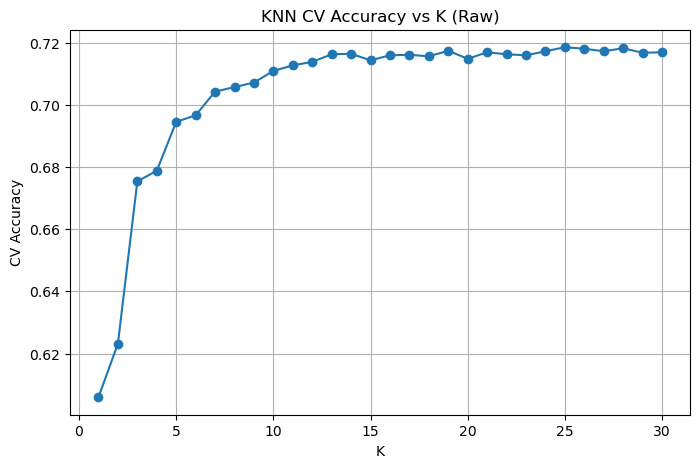
\includegraphics[width=\textwidth]{../results/knn_cs_k_raw.png}
        \caption{KNN hyperparameter tuning for the original dataset.}
        \label{fig:knn_k_tuning_raw}
    \end{subfigure}
    \hfill
    \begin{subfigure}[t]{0.45\textwidth}
        \centering
        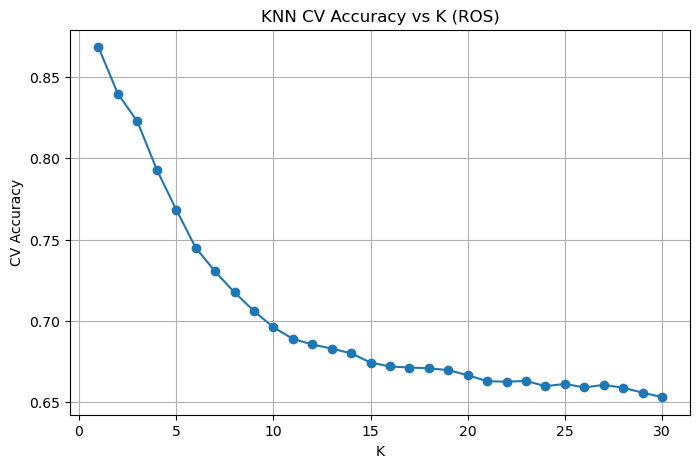
\includegraphics[width=\textwidth]{../results/knn_vs_k_ros.png}
        \caption{KNN hyperparameter tuning for the random oversampling dataset.}
        \label{fig:knn_k_tuning_ros}
    \end{subfigure}
    \vskip\baselineskip
    \begin{subfigure}[t]{0.45\textwidth}
        \centering
        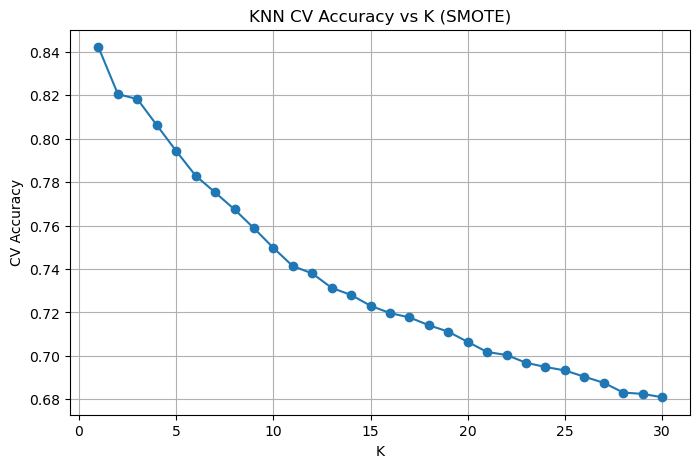
\includegraphics[width=\textwidth]{../results/knn_vs_k_smote.png}
        \caption{KNN hyperparameter tuning for the SMOTE-balanced dataset.}
        \label{fig:knn_k_tuning_smote}
    \end{subfigure}
    \hfill
    \begin{subfigure}[t]{0.45\textwidth}
        \centering
        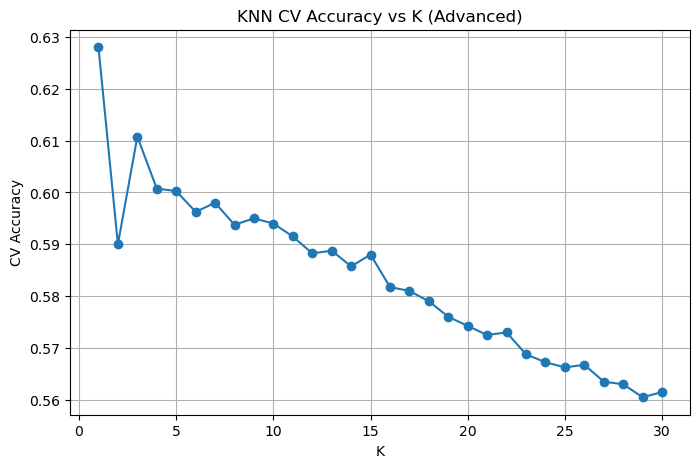
\includegraphics[width=\textwidth]{../results/knn_vs_k_advanced.png}
        \caption{KNN hyperparameter tuning for the advanced-balanced dataset.}
        \label{fig:knn_k_tuning_advanced}
    \end{subfigure}
    \caption{KNN hyperparameter tuning results for different datasets.}
    \label{fig:knn_hyperparameter_tuning}
\end{figure}


\section{Random Forest Optimization and Comparative Evaluation}

\subsection{Hyperparameter Tuning}

\subsection{Random Forest Hyperparameter Tuning}

In Random Forest, different hyperparameters need to be set and evaluated to achieve optimal model performance. Key hyperparameters include the number of trees in the forest (\texttt{n\_estimators}), the number of features considered at each split (\texttt{max\_features}), the maximum depth of each tree (\texttt{max\_depth}), the maximum number of leaf nodes (\texttt{max\_leaf\_nodes}), and the minimum number of samples required at each node (\texttt{min\_samples\_leaf}).

Due to the large number of possible hyperparameter combinations, we applied grid search combined with cross-validation to identify the best-performing configurations. 
A range of values was specified for each parameter. Specifically:

\begin{itemize}
    \item \texttt{n\_estimators}: \{50, 100, 200, 300, 500, 1000\}
    \item \texttt{max\_features}: from 1 to the total number of predictors
    \item \texttt{max\_depth}: \{5, 10, 15, 20, 30, Unlimited\}
    \item \texttt{max\_leaf\_nodes}: \{10, 20, 50, Unlimited\}
    \item \texttt{min\_samples\_leaf}: \{1, 2, 5, 10\}
\end{itemize}

Based on the cross-validation results, the optimal hyperparameter combinations that achieved the 
highest validation accuracy are summarized in Table~\ref{tab:rf_hyperparameters}.
 These findings suggest that different data balancing methods can influence the ideal model complexity and tree structure required for best predictive performance.

    
\begin{table}[!h]
    \centering
    \resizebox{\textwidth}{!}{%
    \begin{tabular}{|l|c|c|c|c|c|}
    \hline
    \textbf{Dataset} & \texttt{n\_estimators} & \texttt{max\_features} & \texttt{max\_depth} & \texttt{max\_leaf\_nodes} & \texttt{min\_samples\_split} \\
    \hline
    Raw & 100 & 6 & 10 & 50 & 1 \\
    Random Oversampling & 300 & 4 & 30 & Unlimited & 1 \\
    SMOTE & 300 & 4 & 30 & Unlimited & 1 \\
    Advanced Sampling & 300 & 4 & 30 & Unlimited & 1 \\
    \hline
    \end{tabular}%
    }
    \caption{Optimal hyperparameters for Random Forest across different datasets.}
    \label{tab:rf_hyperparameters}
\end{table}

\section{Results}

Models were trained and evaluated using accuracy, sensitivity (recall), and specificity:

\begin{align*}
\text{Accuracy} &= \frac{TP + TN}{TP + TN + FP + FN} \\
\text{Sensitivity (Recall)} &= \frac{TP}{TP + FN} \\
\text{Specificity} &= \frac{TN}{TN + FP}
\end{align*}

\subsection{Raw Dataset}

\begin{table}[!h]
\centering
\resizebox{\textwidth}{!}{%
\begin{tabular}{|l|ccc|ccc|ccc|ccc|ccc|}
\hline
\textbf{Model} & \multicolumn{3}{c|}{Class 1} & \multicolumn{3}{c|}{Class 2} & \multicolumn{3}{c|}{Class 3} & \multicolumn{3}{c|}{Class 4} & \multicolumn{3}{c|}{Class 5} \\
& Acc & Sen & Spe & Acc & Sen & Spe & Acc & Sen & Spe & Acc & Sen & Spe & Acc & Sen & Spe \\
\hline
KNN & 0.79 & 0.90 & 0.72 & 0.89 & 0.23 & 0.97 & 0.93 & 0.00 & 1.00 & 1.00 & 0.00 & 1.00 & 0.83 & 0.79 & 0.86 \\
RF & 0.80 & 0.88 & 0.75 & 0.89 & 0.32 & 0.97 & 0.93 & 0.00 & 1.00 & 0.99 & 0.00 & 1.00 & 0.84 & 0.84 & 0.84 \\
\hline
\end{tabular}%
}
\caption{Performance Comparison on Raw Dataset}
\label{tab:raw_dataset_performance}
\end{table}

\subsection{Random Oversampling}

\begin{table}[!h]
\centering
\resizebox{\textwidth}{!}{%
\begin{tabular}{|l|ccc|ccc|ccc|ccc|ccc|}
\hline
\textbf{Model} & \multicolumn{3}{c|}{Class 1} & \multicolumn{3}{c|}{Class 2} & \multicolumn{3}{c|}{Class 3} & \multicolumn{3}{c|}{Class 4} & \multicolumn{3}{c|}{Class 5} \\
& Acc & Sen & Spe & Acc & Sen & Spe & Acc & Sen & Spe & Acc & Sen & Spe & Acc & Sen & Spe \\
\hline
KNN & 0.75 & 0.71 & 0.77 & 0.83 & 0.28 & 0.91 & 0.88 & 0.19 & 0.94 & 0.99 & 0.25 & 0.99 & 0.80 & 0.73 & 0.84 \\
RF & 0.80 & 0.84 & 0.76 & 0.88 & 0.39 & 0.94 & 0.92 & 0.04 & 0.99 & 0.99 & 0.00 & 1.00 & 0.84 & 0.81 & 0.86 \\
\hline
\end{tabular}%
}
\caption{Performance Comparison on Random Oversampling Dataset}
\label{tab:random_oversampling_performance}
\end{table}

\subsection{SMOTE}

\begin{table}[!h]
\centering
\resizebox{\textwidth}{!}{%
\begin{tabular}{|l|ccc|ccc|ccc|ccc|ccc|}
\hline
\textbf{Model} & \multicolumn{3}{c|}{Class 1} & \multicolumn{3}{c|}{Class 2} & \multicolumn{3}{c|}{Class 3} & \multicolumn{3}{c|}{Class 4} & \multicolumn{3}{c|}{Class 5} \\
& Acc & Sen & Spe & Acc & Sen & Spe & Acc & Sen & Spe & Acc & Sen & Spe & Acc & Sen & Spe \\
\hline
KNN & 0.75 & 0.64 & 0.82 & 0.81 & 0.30 & 0.88 & 0.85 & 0.24 & 0.90 & 0.98 & 0.25 & 0.98 & 0.80 & 0.71 & 0.87 \\
RF & 0.80 & 0.79 & 0.80 & 0.86 & 0.39 & 0.92 & 0.89 & 0.09 & 0.96 & 0.99 & 0.12 & 1.00 & 0.84 & 0.79 & 0.87 \\
\hline
\end{tabular}%
}
\caption{Performance Comparison on SMOTE Dataset}
\label{tab:smote_dataset_performance}
\end{table}

\subsection{Advanced Sampling}

\begin{table}[!h]
\centering
\resizebox{\textwidth}{!}{%
\begin{tabular}{|l|ccc|ccc|ccc|ccc|ccc|}
\hline
\textbf{Model} & \multicolumn{3}{c|}{Class 1} & \multicolumn{3}{c|}{Class 2} & \multicolumn{3}{c|}{Class 3} & \multicolumn{3}{c|}{Class 4} & \multicolumn{3}{c|}{Class 5} \\
& Acc & Sen & Spe & Acc & Sen & Spe & Acc & Sen & Spe & Acc & Sen & Spe & Acc & Sen & Spe \\
\hline
KNN & 0.72 & 0.54 & 0.84 & 0.78 & 0.36 & 0.84 & 0.82 & 0.27 & 0.86 & 0.97 & 0.25 & 0.98 & 0.79 & 0.65 & 0.88 \\
RF & 0.79 & 0.72 & 0.83 & 0.84 & 0.51 & 0.89 & 0.88 & 0.12 & 0.94 & 0.99 & 0.12 & 1.00 & 0.84 & 0.76 & 0.88 \\
\hline
\end{tabular}%
}
\caption{Performance Comparison on Advanced Sampling Dataset}
\label{tab:advanced_sampling_performance}
\end{table}

\subsection{Summary}

Among all methods, \textbf{KNN with SMOTE} provided the best sensitivity on minority classes, particularly Class 3 and 4, while maintaining acceptable accuracy on majority classes. However, sensitivity values around 25\% still indicate room for improvement in detecting rare but clinically important conditions.
\section{Bayesian Improved Logistic Regression}

In this section, we will try to create a Bayesian improved logistic regression using splines.
The ideas is to use the splines to model the non-linear relationship between the variables and the response variables.
Instead of using the classical statistical methods - Maximum Likelihood Estimation (MLE) to 
estimate the parameters of the model, we will use the Bayesian approach to estimate the posterior distribution of the parameters.
The predicated probability of the target variable being 1 will be a distribution 
up to the posterior distribution of the parameters and the final predicted label will depend on the expectation of 
the posterior distribution.


\subsection{Transfomation on design matrix for regression splines}

Regression splines is a powerful tool to model the non-linear relationship 
between the input variables and the response variable. It splits the input space into 
several intervals and fits basis functions to each interval. The basis functions can 
be choosen to be simple linear or polynomial functions, or more complex functions. 
The functions across the intervals are connected at the knots, which makes sure 
the total regression function is continuous and smooth.

Given a univariate predictor $x \in {R}^n$, we can construct a regression spline design matrix by transforming $x$ into a set of basis functions. For a spline of degree $d$ with $K$ knots $\{\xi_1, \xi_2, \dots, \xi_K\}$, the new design matrix $\mathbf{X}_{\text{spline}}$ is:

\[
\mathbb {K}:  X (n,p) \mapsto X_{spline}(n, p + C), \quad C > 1
\]

\[
\mathbf{X}_{\text{spline}} = 
\begin{bmatrix}
1 & x_{11} & x_{11}^2  & x_{21} & x_{21}^2  & \cdots & x_{p1}^d & (x_{11} - \xi_{11})_+^d & \cdots & (x_{p1} - \xi_{pK})_+^d \\
1 & x_{12} & x_{12}^2  & x_{22} & x_{22}^2 & \cdots & x_{p2}^d & (x_{12} - \xi_{11})_+^d & \cdots & (x_{p2} - \xi_{pK})_+^d \\
\vdots & \vdots  & \vdots & \vdots & \vdots & & \vdots & \vdots & & \vdots \\
1 & x_{1n} & x_{1n}^2  & x_{2n} & x_{2n}^2 & \cdots & x_{pn}^d & (x_{1n} - \xi_{11})_+^d & \cdots & (x_{pn} - \xi_{pK})_+^d \\
\end{bmatrix}
\]

Here, $(x - \xi_j)_+^d$ denotes the truncated power basis function:
\[
(x - \xi_j)_+^d = 
\begin{cases}
(x - \xi_j)^d & \text{if } x > \xi_j \\
0 & \text{otherwise}
\end{cases}
\]

This design matrix allows the regression model to fit a flexible, 
piecewise polynomial function with continuity at the specified knots.

\subsection{The likelihood function of $\beta$ in the logistic regression}

To a data set having target variable that has only two vlaues, we view the target variable follows a Bernoulli distribution with
true parameter $p$. The parameter is the probability of the target variable being 1 and is determined by 
the linear combination of the input variables $X$ and the parameters $\beta$. It gives: \(Y_i \sim Bernoulli(p_i)\).

By linking function - \(log(\frac{x}{1-x})\), the conditional probability of the target variable $Y$ given the input variables $X$ is given by
\footnote{$\frac{p}{1-p}$ is doing broadcast operation, which makes sure the result is still a vector 
not linear algebra dot product.}:
\[
log(\frac{p}{1-p}) = X \beta, 
\]

Where \(p\) is the vector of true predicted probabiltiy of \(Y\) being 1, \(X\) is design matrix of the input variables, 
and \(\beta\) is the vector of the parameters.


\[
p = \begin{bmatrix} p_1 \\ p_2 \\ \vdots \\ p_n \end{bmatrix}, \quad
X = \begin{bmatrix} X_{11} & X_{12} & \cdots & X_{1p} \\ X_{21} & X_{22} & \cdots & X_{2p} \\ \vdots & \vdots & \ddots & \vdots \\ X_{n1} & X_{n2} & \cdots & X_{np} \end{bmatrix}, \quad
\beta = \begin{bmatrix} \beta_1 \\ \beta_2 \\ \vdots \\ \beta_p \end{bmatrix}.
\]

After taking the inverse of the link function, we can get the predicted probability of the target variable being 1
\footnote{'$\sigma$' is a sigmoid function, which takes \(X\) and \(\beta\) as input and returns the predicted probability,
we will use it later for simplicity.}:

\[
p = \sigma(X, \beta) = \frac{1}{1+e^{-X\beta}}.
\]

Based on the above probability model, we can get the likelihood function 
of parameters \(\beta\) given the data set \((X, Y)\):
\[
L(\beta|X, Y) = \prod_{i=1}^n p_i^{Y_i} (1-p_i)^{1-Y_i} \tag{1-1}
\]

% Instead of using the multiplication form to consider the likelihood of the data set, we can also use 
% addition form to calculate it:
% \[
% L(\beta|X, Y) = \prod_{i=1}^n ( {Y_i}  p_i + ({1-Y_i})(1-p_i) )\tag{2-1}
% \]

Taking logarithm of the likelihood function and replacing \(p_i\) with 
\(\sigma(X_i, \beta)\)\footnote{$X_i$ is the input vector of \(i\)th observation.}, 
we can get the log-likelihood function of the parameters \(\beta\) given the data set \((X, Y)\):

\begin{align*}
    \ell_n(\beta) 
    & = \sum_{i=1}^n [y_i log(\sigma(x_i, \beta)) + (1-y_i) log(1-\sigma(x_i, \beta))] \\
    & = \sum_{i=1}^n (x_iy_i \beta - log(1+e^{x_i\beta}))
\end{align*}


We search for the maximum of the log-likelihood function to get the MLE of the parameters \(\beta\):
\[
\hat{\beta} = \arg\max_{\beta} \ell_n(\beta)
\]

To find a good solution for the MLE, we can use the Newton-Raphson method to iteratively update the parameters \(\beta\):
\[
\beta_{k+1} = \beta_k - H^{-1}(\beta_k) \nabla \ell_n(\beta_k)
\]

Where \(H(\beta_k)\) is the Hessian matrix of the log-likelihood function \(\ell_n(\beta)\) at \(\beta_k\), 
and \(\nabla \ell_n(\beta_k)\) is the gradient vector of the log-likelihood function \(\ell_n(\beta)\) at \(\beta_k\).
The initial value of \(\beta\) can be set to any proper value, but a good choice can accelerate the convergence speed.

The Hessian matrix and the gradient vector can be calculated as follows
\footnote{We assume the \(X's\) are independent that we can add n individual observed 
Fisher information to get the total Fisher information. \(H\) is summation of n matrices in \((p, p)\) ,
$\nabla \ell_n(\beta)$ is the vector of the first derivative of the log-likelihood function}:

\begin{align*}
    H(\beta) & = -\sum_{i=1}^n \sigma(x_i, \beta)(1-\sigma(x_i, \beta))x_ix_i^T \\
    \nabla \ell_n(\beta) & = \sum_{i=1}^n (y_i - \sigma(x_i, \beta))x_i
\end{align*}

\subsection{Prior about $\beta$ from bootstrapping method}

In situations where prior information about the regression coefficients
 $\boldsymbol{\beta}$ is unavailable or limited, 
a data-driven approach can be employed by using the bootstrap method to approximate
 the sampling distribution of $\boldsymbol{\beta}$. Specifically, we perform repeated 
 sampling with replacement from the observed dataset and estimate $\boldsymbol{\beta}$ 
 for each bootstrap replicate using a frequentist method such as ordinary least squares. 
 This yields a collection of $\boldsymbol{\beta}$ estimates, from which we can compute 
 the empirical mean $\hat{\boldsymbol{\beta}}$ and covariance matrix $\Sigma_{\text{boot}}$. 
 These estimates can then be used to define an informative multivariate normal prior for
  Bayesian inference:

\[
\boldsymbol{\beta} \sim \mathcal{N}(\hat{\boldsymbol{\beta}}, \Sigma_{\text{boot}})
\]

This bootstrap-based prior reflects the variability observed in the data and provides 
a pragmatic empirical Bayes approach. While it does not represent a fully Bayesian treatment 
(as the prior is derived from the data), it enables regularization and uncertainty quantification 
in a principled way.

\subsection{Bayesian improved logistic regression}
After getting the likelihood function or \(\beta\) from original data
 and prior distribution of \(\beta\) from bootstrapping method,
we can use the Bayes' theorem to get the posterior distribution of \(\beta\):
\[
\mathbb P(\beta|X, Y) = \frac{L(\beta|X, Y) p(\beta)}{p(X, Y)} \tag{1-2}
\]

Where \(p(X, Y)\) is the marginal likelihood of the data set \((X, Y)\). 

The posterior does not belong to any known distribution, but it is proportional to its numerator
\(p_{\beta_{post}} =\mathbb P (\boldsymbol{\beta} \mid \mathbf{y}, \mathbf{X}) \):
\[
\mathbb P (\boldsymbol{\beta} \mid \mathbf{y}, \mathbf{X}) \propto \ell_n(\beta) \cdot p(\beta)
\]

it gives that we can get the 95\% credible interval of \(\beta\) from this 
proportional unnormalized posterior distribution.

Based on the unnormalized distribution of \(\beta\), 
we can get the posterior predictive distribution of the prability of 
target variable \(Y\) given the input variables \(X\):
\[
\mathbb P_{Y_{[\alpha, 1- \alpha]}} = [X \beta_{\alpha}, X \beta_{1 - \alpha}]
\]

We set the probability of \(Y\) being 1 as the mean of the posterior predictive distribution of \(Y\):
\[
\mathbb P_{Y=1} = E[\beta_{post} X] = \frac{1}{B} \sum_{b=1}^B \sigma(X, \beta_b)
\]

This modular design enables robust inference, handles nonlinearities via splines, and leverages empirical Bayesian estimation through bootstrapped priors.

\subsection{One-VS-Rest classification}

We use one-vs-rest method to transit from binary logistic regression to multi-class classification.

The logistic regression model for class \(k\) predicts the probability of an observation belonging to class \(k\) as:
\[
P(y = k \mid \mathbf{x}) = \sigma(\mathbf{x} \boldsymbol{\beta}^{(k)}) = \frac{1}{1 + e^{-\mathbf{x} \boldsymbol{\beta}^{(k)}}},
\]
where \(\boldsymbol{\beta}^{(k)}\) is the parameter vector for class \(k\).

After training all \(K\) models, the predicted class for a new observation \(\mathbf{x}\) is determined by selecting the class with the highest predicted probability:
\[
\hat{y} = \arg\max_{k \in \{1, 2, \dots, K\}} P(y = k \mid \mathbf{x}).
\]

This approach allows binary logistic regression to handle multi-class problems by leveraging the simplicity of binary classification while maintaining interpretability and flexibility.


\subsection{Implementation of deriving Prior Distribution of $\beta$}

To make the modling work simpler, we only use the data set processed by SMOTE method for work in this 
section.





\begin{figure}[!h]
    \centering
    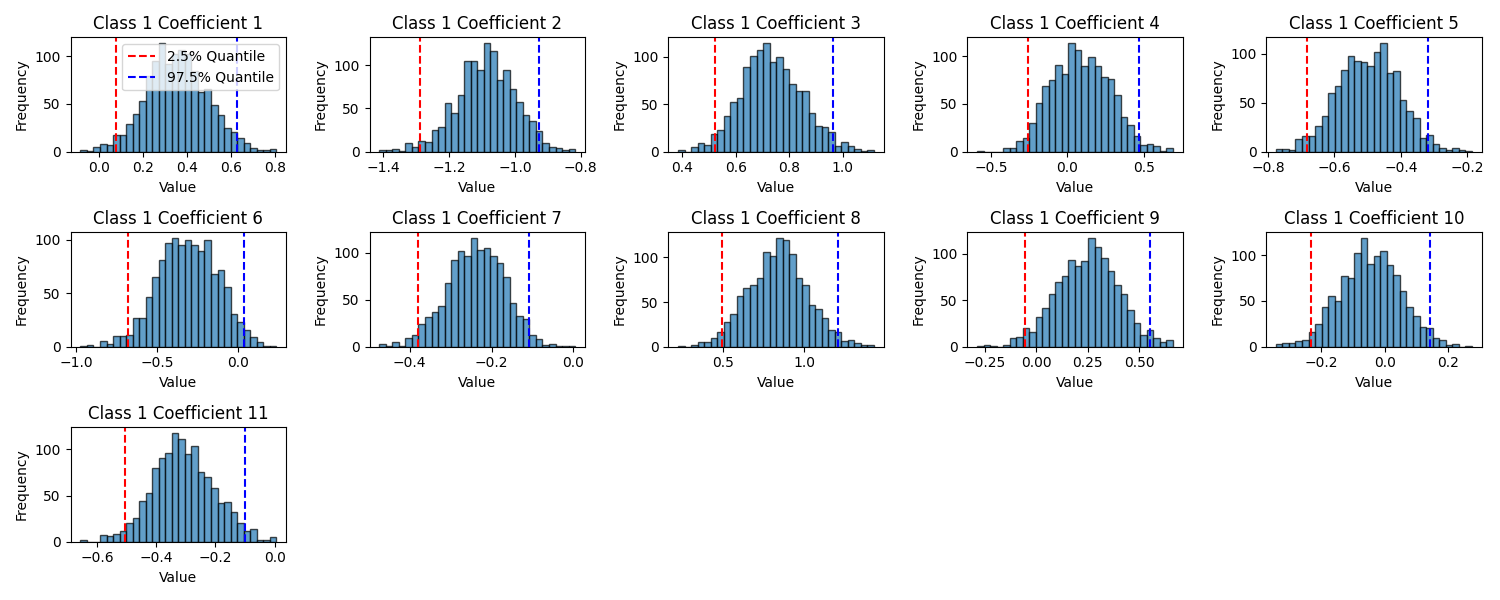
\includegraphics[width=1\textwidth]{../results/ModelFitting2/bootstrap_estimates_histograms.png}
    \caption{Bootstrap estimates histograms for prior distribution of $\beta_i$}
    \label{fig:bootstrap_estimates_histograms}
\end{figure}

Figure~\ref{fig:bootstrap_estimates_histograms}
\footnote{Here we only use class 1 in response variable to demonstrate how we obtain the distribution of 
$\beta_i$ from bootstrap method, that's there is 'Class 1' string in titles.} 
shows the empirical prior distributions of the
logistic regression coefficients $\beta_i$ estimated using bootstrap
resampling for class label 1 among the five target categories.
Each subplot corresponds to a coefficient in the model, including the intercept term. 

The histograms represent the frequency distribution of coefficient estimates across 
bootstrap samples, giving an approximation of the sampling distribution under repeated sampling. 
Vertical dashed lines mark the 2.5\% and 97.5\% quantiles, providing a 95\% empirical confidence 
interval for each $\beta_i$. These intervals reflect the uncertainty of the coefficients prior 
to incorporating the likelihood in the Bayesian inference step.

\begin{figure}[!h]
    \centering
    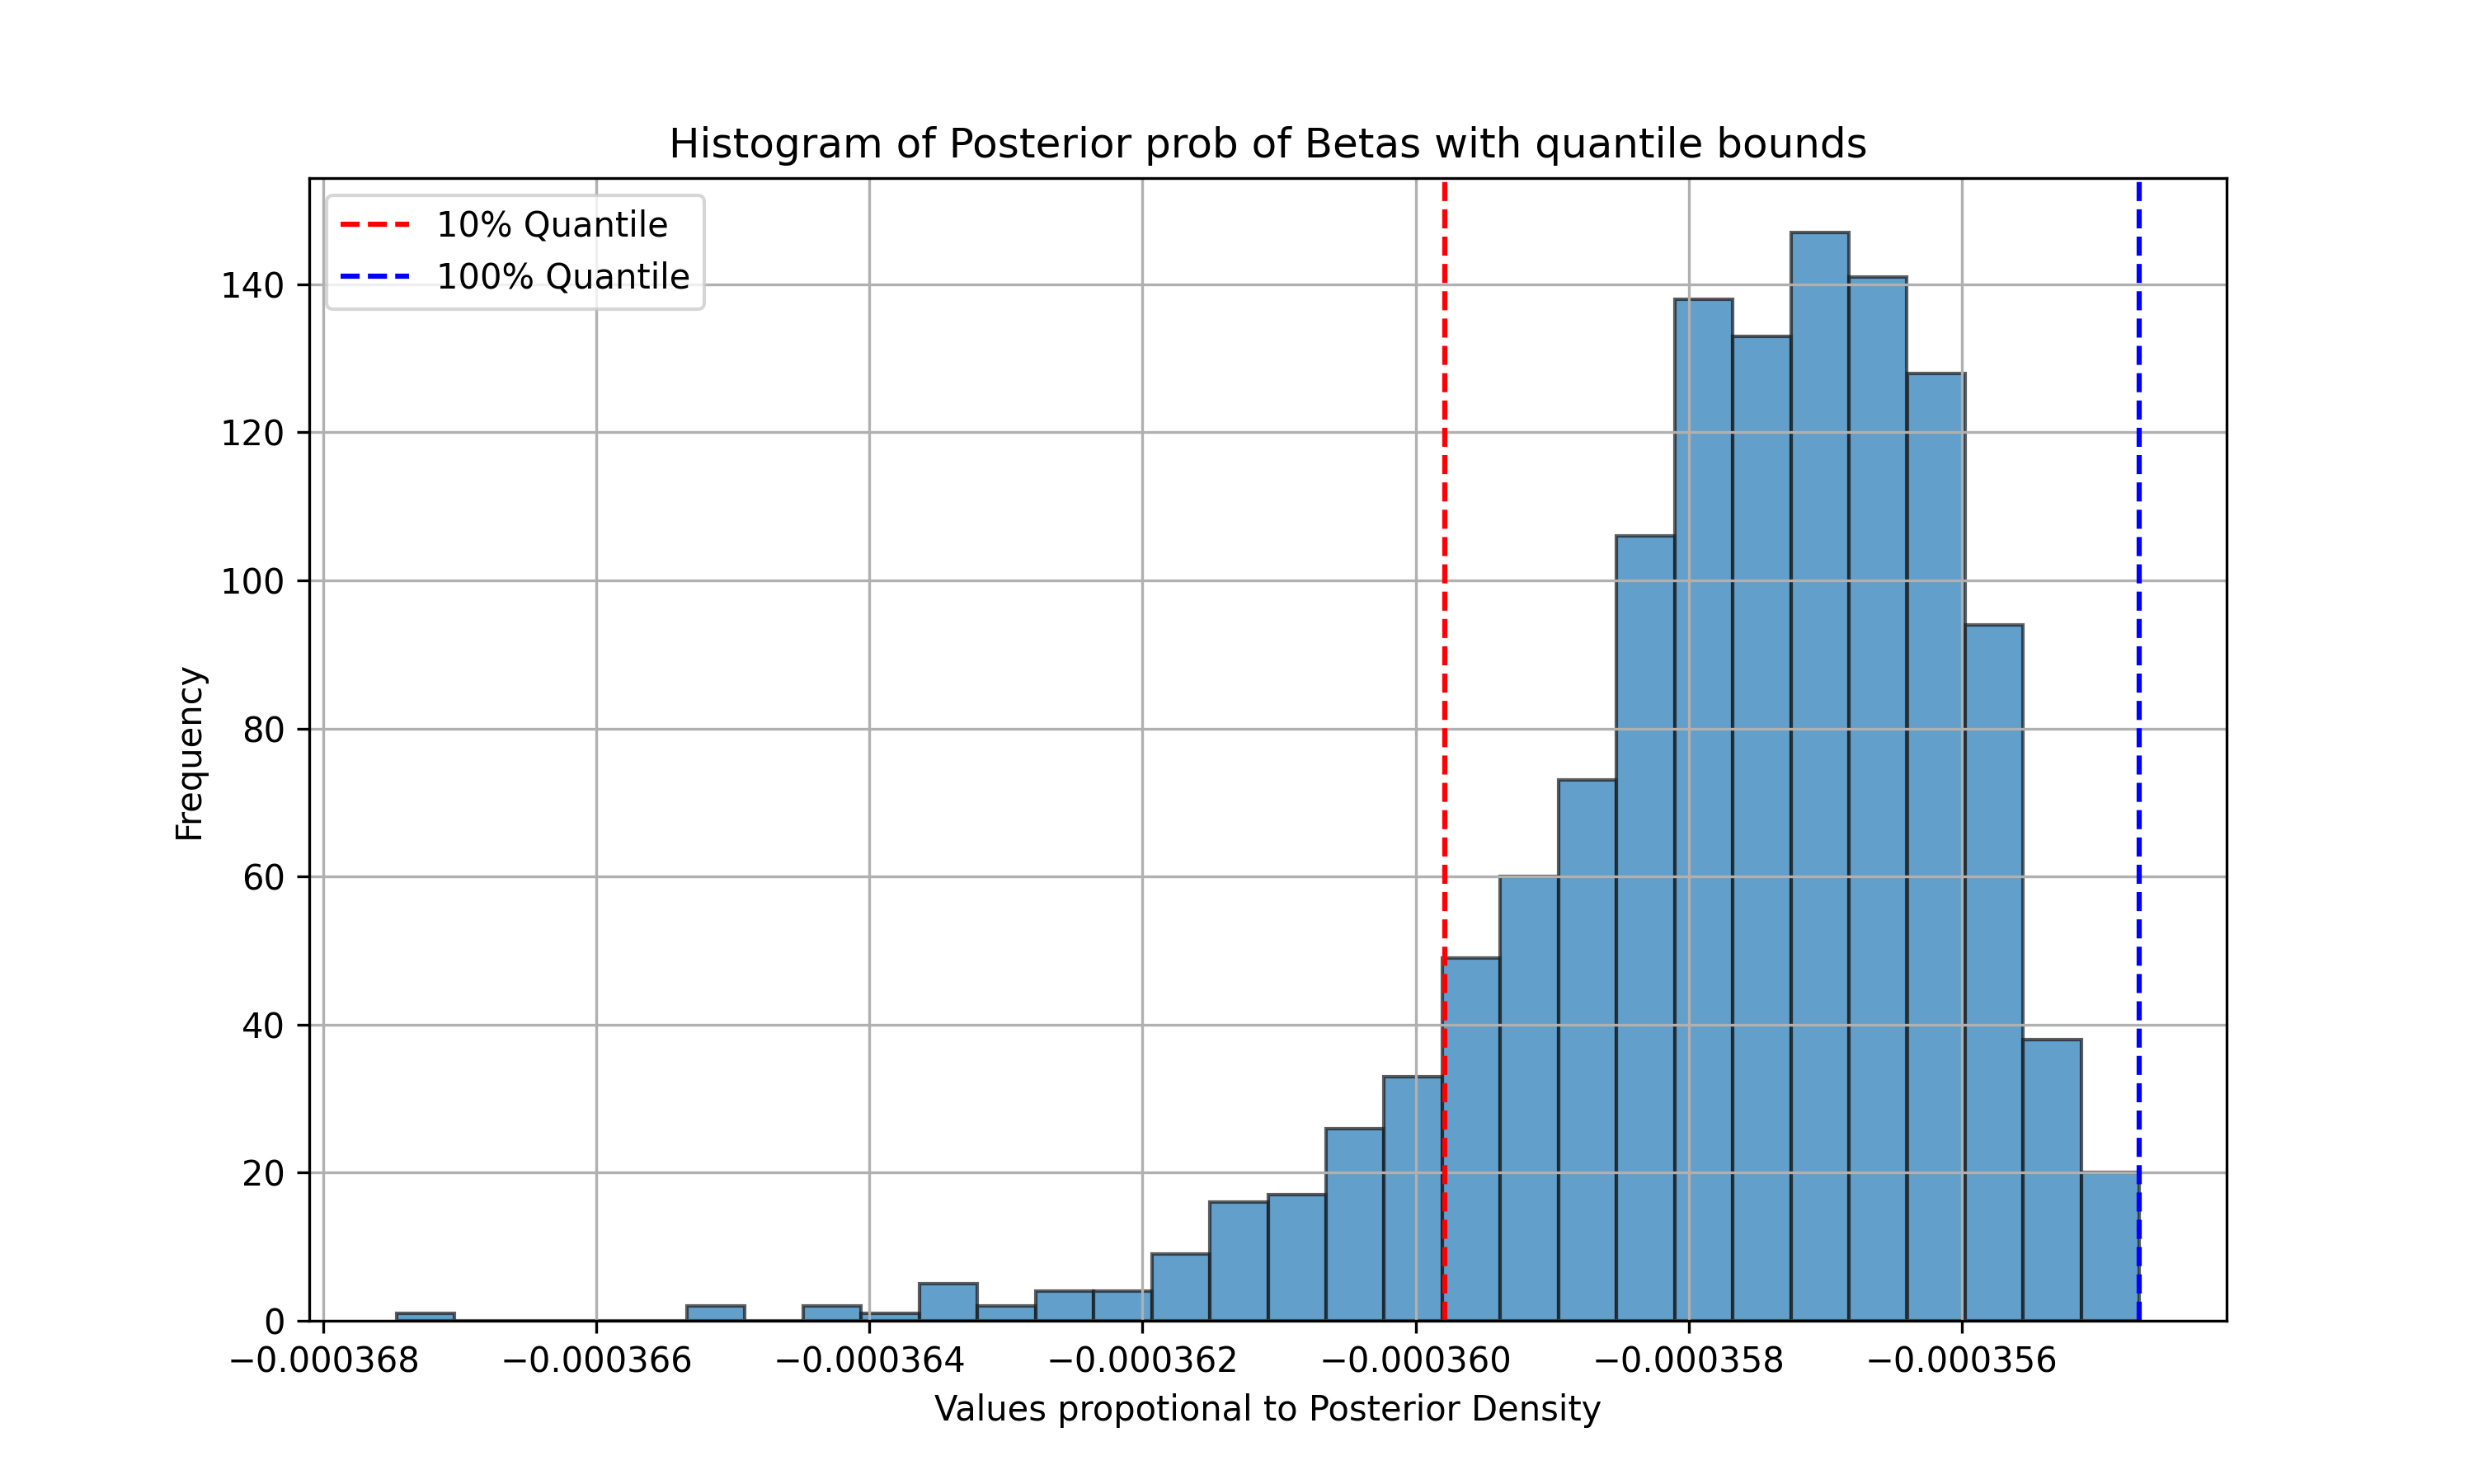
\includegraphics[width=0.9\textwidth]{../results/ModelFitting2/bayesian_posterior_density_histogram.png}
    \caption{Hist of values proportional to the posterior distribution of $\beta$ vector}
    \label{fig:bayesian_posterior_density_histogram}
\end{figure}

Figure~\ref{fig:bayesian_posterior_density_histogram} shows the histogram of values proportional to the posterior distribution of the logistic regression coefficients $\beta$. These values represent the product of the likelihood and the bootstrap-estimated prior, up to a normalization constant.

The vertical dashed lines indicate the 10\% and 100\% quantile thresholds, 
highlighting the top 90\% of posterior-proportional values. 
This range identifies the most probable $\beta$ candidates,
 useful for summarizing the posterior or computing the expected $\beta$
 \footnote{The computation is also based on class 1 among the 5 classes.}.

\subsection{Model performance evaluation}

After repeatedly training the model on 5 different classes, we can get the 
model performance metrics of the models.

Table ~\ref{tab:metrics_train} shows the model performance metrics of the performance of bayesian logsistic regression  
and MLE logistic regression model on training data.

\begin{table}[!h]
    \centering
    \caption{Model evaluation metrics grouped by target}
    \label{tab:metrics_train}
    \begin{tabular}{cccccc}
    \toprule
    \textbf{Target} & \textbf{Accuracy} & \textbf{Precision} & \textbf{Recall} & \textbf{F1 Score} & \textbf{Model} \\
    \midrule
    \multirow{2}{*}{1} & 0.8629 & 0.6111 & 0.8800 & 0.7213 & MLE \\
                       & 0.8629 & 0.6111 & 0.8800 & 0.7213 & Bayesian \\
    \midrule
    \multirow{2}{*}{2} & 0.6774 & 0.3729 & 0.8800 & 0.5238 & MLE \\
                       & 0.7016 & 0.3889 & 0.8400 & 0.5316 & Bayesian \\
    \midrule
    \multirow{2}{*}{3} & 0.6694 & 0.3095 & 0.5200 & 0.3881 & MLE \\
                       & 0.6855 & 0.3158 & 0.4800 & 0.3810 & Bayesian \\
    \midrule
    \multirow{2}{*}{4} & 0.6048 & 0.2549 & 0.5417 & 0.3467 & MLE \\
                       & 0.6774 & 0.3095 & 0.5417 & 0.3939 & Bayesian \\
    \midrule
    \multirow{2}{*}{5} & 0.7097 & 0.4000 & 0.8800 & 0.5500 & MLE \\
                       & 0.7419 & 0.4186 & 0.7200 & 0.5294 & Bayesian \\
    \bottomrule
    \end{tabular}
\end{table}

Table~\ref{tab:metrics_train} compares the performance of MLE and Bayesian logistic 
regression models on the training dataset across five target classes using standard 
classification metrics. Overall, both models exhibit consistent performance on class 1,
 achieving high accuracy (0.8629), precision (0.6111), recall (0.8800), and F1 score (0.7213),
  suggesting this class is well modeled.

For the remaining classes, Bayesian models tend to slightly outperform MLE models
 in terms of accuracy, precision, and F1 score. For example, in class 2, the Bayesian 
 model achieves higher accuracy (0.7016 vs.\ 0.6774) and better F1 score (0.5316 vs.\ 0.5238),
  despite both models showing strong recall (above 0.84).
   This trend continues in classes 3 and 4, where the Bayesian model improves
    on accuracy and precision, although the recall values remain close.
     Class 4 shows a notable improvement in accuracy (0.6774 vs.\ 0.6048) 
     and F1 score (0.3939 vs.\ 0.3467) for the Bayesian model.

In class 5, the Bayesian model again achieves higher accuracy (0.7419 vs.\ 0.7097), 
although its recall drops slightly compared to MLE (0.7200 vs.\ 0.8800), leading to a
 marginally lower F1 score. Overall, the Bayesian approach generally improves model 
 robustness across imbalanced classes by balancing precision and recall more effectively, 
 as reflected in consistently stronger F1 scores in most classes.


 \begin{table}[!h]
    \centering
    \caption{Model evaluation metrics on test data}
    \label{tab:metrics_test}
    \begin{tabular}{cccccc}
    \toprule
    \textbf{Target} & \textbf{Accuracy} & \textbf{Precision} & \textbf{Recall} & \textbf{F1 Score} & \textbf{Model} \\
    \midrule
    \multirow{2}{*}{1} & 0.5887 & 0.1389 & 0.2000 & 0.1639 & MLE \\
                       & 0.5887 & 0.1389 & 0.2000 & 0.1639 & Bayesian \\
    \midrule
    \multirow{2}{*}{2} & 0.4839 & 0.1695 & 0.4000 & 0.2381 & MLE \\
                       & 0.5081 & 0.1897 & 0.4400 & 0.2651 & Bayesian \\
    \midrule
    \multirow{2}{*}{3} & 0.5403 & 0.1190 & 0.2000 & 0.1493 & MLE \\
                       & 0.5645 & 0.1081 & 0.1600 & 0.1290 & Bayesian \\
    \midrule
    \multirow{2}{*}{4} & 0.5565 & 0.1961 & 0.4167 & 0.2667 & MLE \\
                       & 0.5968 & 0.1905 & 0.3333 & 0.2424 & Bayesian \\
    \midrule
    \multirow{2}{*}{5} & 0.4516 & 0.1091 & 0.2400 & 0.1500 & MLE \\
                       & 0.5323 & 0.1333 & 0.2400 & 0.1714 & Bayesian \\
    \bottomrule
    \end{tabular}
\end{table}

The evaluation on test data reveals a noticeable drop in performance for both models across 
all metrics. Accuracy ranges from approximately 45\% to 59\%, and F1 scores remain low,
 mostly under 0.27. This indicates challenges in generalizing beyond the training data. 
 Despite the overall low performance, the Bayesian model generally achieves slightly 
 higher F1 scores than MLE, particularly for targets 2, 4, and 5,
 suggesting better balance between precision and recall under uncertainty.


\begin{figure}[!h]
    \centering
    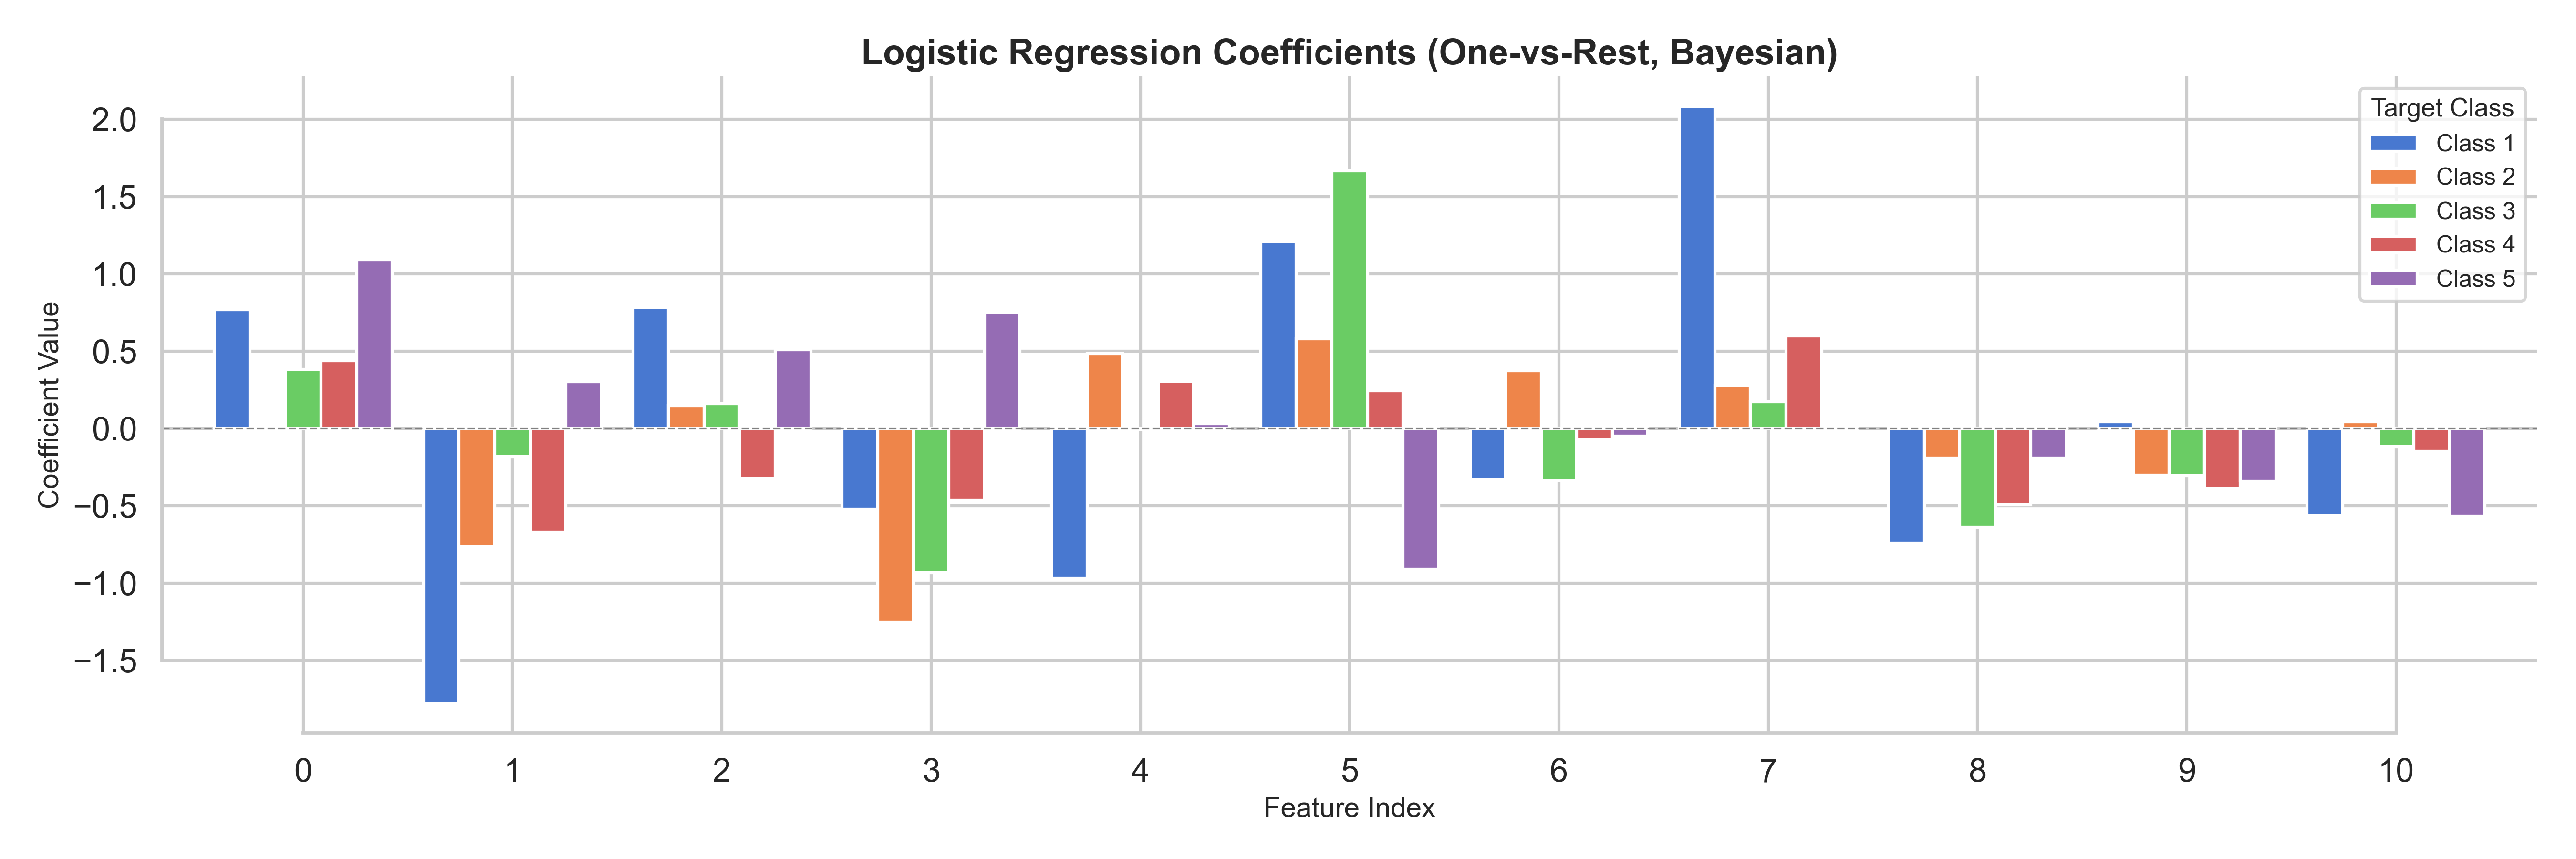
\includegraphics[width=0.9\textwidth]{../results/ModelFitting2/bayesian_coef_plot.png}
    \caption{The importance of each feature in the Bayesian logistic regression model}
    \label{fig:bayesian_coef_plot}
\end{figure}

Figure~\ref{fig:bayesian_coef_plot} illustrates the coefficients 
from five one-vs-rest Bayesian logistic regression models, each targeting a different class. 
Features with large absolute coefficient values have a stronger influence on the model's predictions.
 Notably, features indexed at 0, 1, 5, and 7 exhibit substantial variability across classes, 
 indicating their high discriminative power. For instance, feature 6 is particularly important
  for Class~1 and Class~4, while feature 5 plays a dominant role in Class~3. Conversely, 
  features 8--10 show relatively small coefficients across all classes, suggesting limited 
  influence on prediction. The direction (sign) of each coefficient also reveals whether a 
  feature increases or decreases the likelihood of the corresponding class.

\begin{figure}[!h]
    \centering
    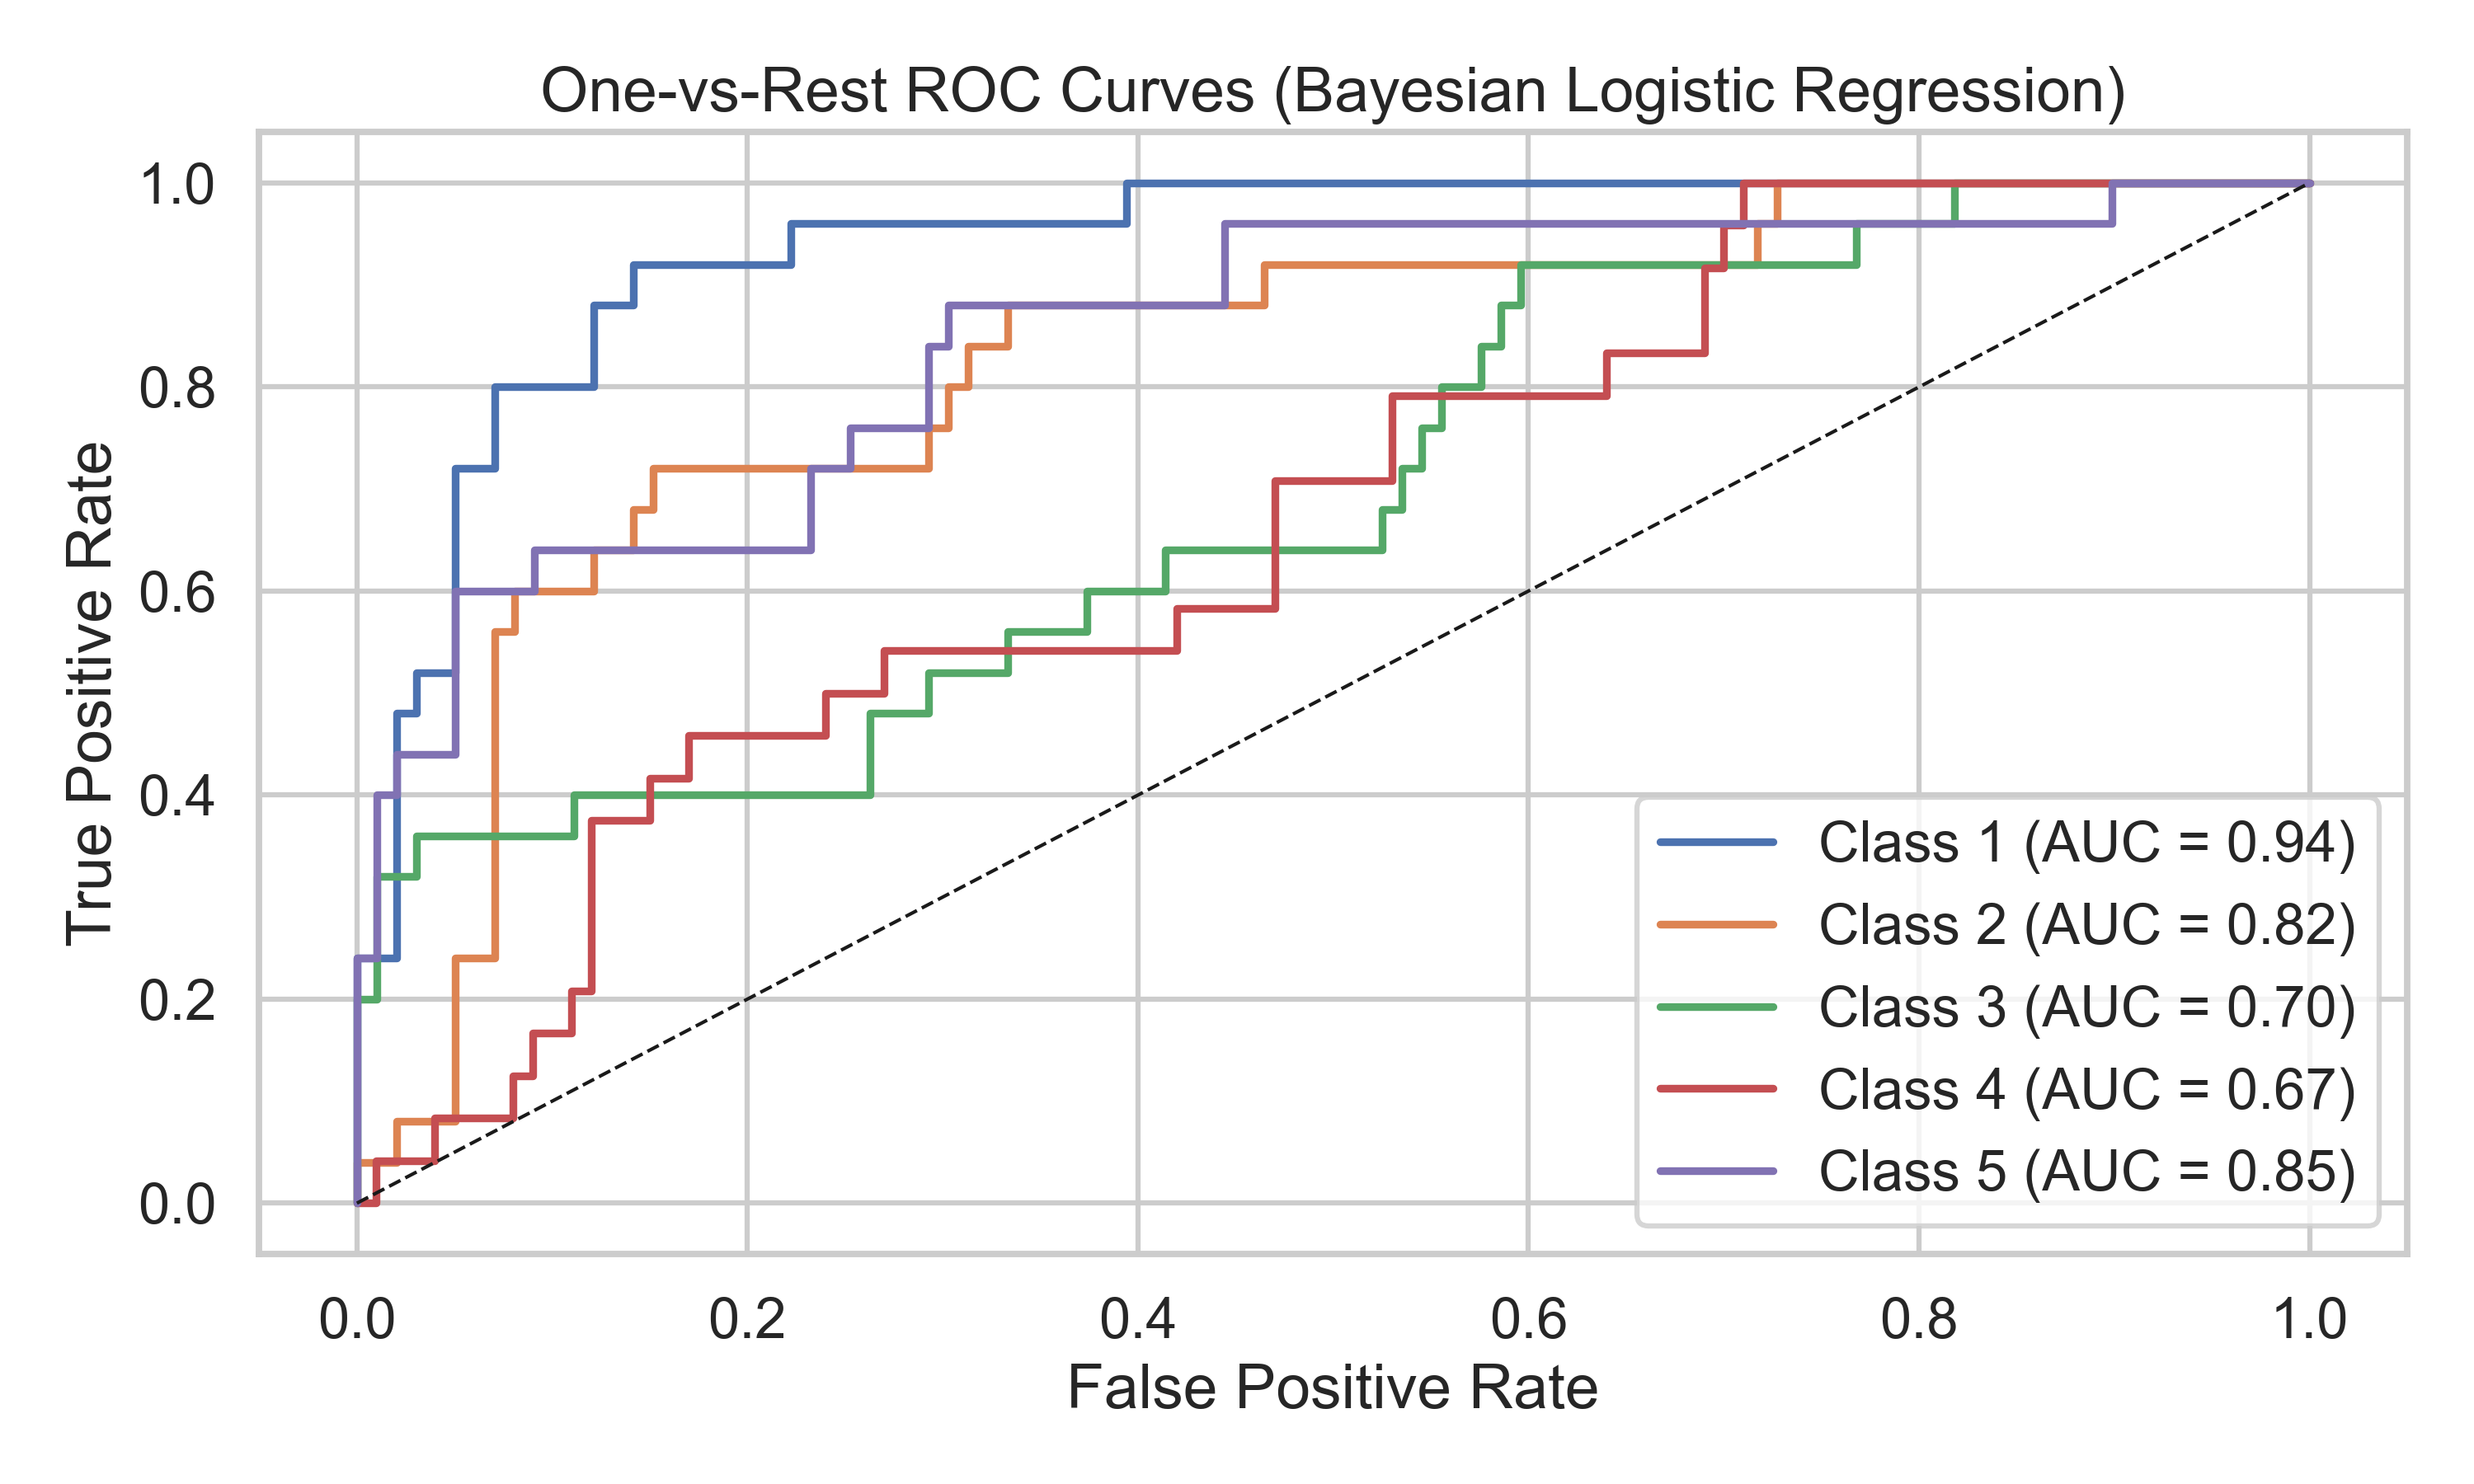
\includegraphics[width=0.9\textwidth]{../results/ModelFitting2/roc_curve_bayesian.png}
    \caption{ROC curve of each of the Bayesian logistic regression models across 5 classes}
    \label{fig:roc_curve_bayesian}
\end{figure}

Figure~\ref{fig:roc_curve_bayesian} displays the ROC curves for the five one-vs-rest Bayesian logistic regression models, each classifying one of the five target classes. 
The Area Under the Curve (AUC) serves as a summary of model performance, where higher values indicate better discrimination. Class~1 achieves the highest AUC (0.94),
 suggesting strong predictive performance. 
Class~5 and Class~2 also show good separation with AUCs of 0.85 and 0.82, respectively. In contrast, Class~3 (AUC = 0.70) and especially Class~4 (AUC = 0.67) demonstrate more 
limited classification ability, with curves closer to the diagonal, indicating greater confusion between classes. Overall, the ROC analysis highlights varying levels of model effectiveness across classes.



\clearpage
% % Bibliography section
\begin{thebibliography}{99} % The number specifies the width of the label

  \bibitem{example1}
  H. Hyndman and G. Athanasopoulos. 
  ``STL Decomposition,'' 
  \textit{Forecasting: Principles and Practice (3rd ed.)}. 
  Available at: \url{https://otexts.com/fpp3/stl.html}. 
  Accessed: November 30, 2024.

\end{thebibliography}
% \section{Appendix}

\subsection{Tables}

% \begin{table}[!h]
%     \centering
%     \caption{Variable descriptions in the SUPPORT2 dataset.}
%     \label{tab:metrics}
%     \begin{tabular}{cccccccccccc}
%     \toprule
%     \textbf{index} & \textbf{count} & \textbf{mean} & \textbf{std} & \textbf{min} & \textbf{25\%} & \textbf{50\%} & \textbf{75\%} & \textbf{max} & \textbf{skewness} & \textbf{kurtosis} & \textbf{shapiro-p} \\
%     \midrule
%     age & 6164.00 & 62.85 & 15.72 & 18.12 & 53.03 & 65.02 & 74.38 & 100.85 & -0.52 & -0.15 & 0.00 \\
%     death & 6164.00 & 0.70 & 0.46 & 0.00 & 0.00 & 1.00 & 1.00 & 1.00 & -0.88 & -1.23 & 0.00 \\
%     hospdead & 6164.00 & 0.30 & 0.46 & 0.00 & 0.00 & 0.00 & 1.00 & 1.00 & 0.88 & -1.23 & 0.00 \\
%     slos & 6164.00 & 17.38 & 20.89 & 3.00 & 6.00 & 11.00 & 19.00 & 343.00 & 4.53 & 33.64 & 0.00 \\
%     d.time & 6164.00 & 439.63 & 549.71 & 3.00 & 19.00 & 164.00 & 692.25 & 2029.00 & 1.31 & 0.66 & 0.00 \\
%     num.co & 6164.00 & 1.89 & 1.36 & 0.00 & 1.00 & 2.00 & 3.00 & 9.00 & 0.83 & 0.65 & 0.00 \\
%     edu & 5330.00 & 11.72 & 3.44 & 0.00 & 10.00 & 12.00 & 14.00 & 31.00 & -0.08 & 1.46 & 0.00 \\
%     scoma & 6163.00 & 13.07 & 25.88 & 0.00 & 0.00 & 0.00 & 9.00 & 100.00 & 2.21 & 4.13 & 0.00 \\
%     charges & 6046.00 & 58803.09 & 98338.95 & 1169.00 & 10074.50 & 25471.50 & 63906.00 & 1226766.00 & 4.58 & 30.48 & 0.00 \\
%     totcst & 5538.00 & 30783.65 & 45256.68 & 0.00 & 6135.76 & 14735.33 & 36022.55 & 483556.25 & 3.88 & 21.95 & 0.00 \\
%     totmcst & 3830.00 & 28725.87 & 43705.41 & -102.72 & 5405.90 & 13600.49 & 33526.49 & 710682.00 & 4.75 & 39.21 & 0.00 \\
%     avtisst & 6115.00 & 23.22 & 13.50 & 1.00 & 12.00 & 20.33 & 32.67 & 83.00 & 0.72 & -0.17 & 0.00 \\
%     sps & 6163.00 & 26.04 & 10.08 & 0.20 & 19.40 & 24.30 & 30.75 & 99.19 & 1.58 & 5.31 & 0.00 \\
%     aps & 6163.00 & 38.71 & 20.33 & 1.00 & 24.00 & 35.00 & 50.00 & 143.00 & 0.92 & 0.92 & 0.00 \\
%     surv2m & 6163.00 & 0.62 & 0.26 & 0.00 & 0.48 & 0.70 & 0.82 & 0.97 & -0.95 & -0.10 & 0.00 \\
%     surv6m & 6163.00 & 0.51 & 0.26 & 0.00 & 0.31 & 0.56 & 0.72 & 0.95 & -0.48 & -0.90 & 0.00 \\
%     hday & 6164.00 & 4.55 & 9.43 & 1.00 & 1.00 & 1.00 & 4.00 & 148.00 & 6.07 & 57.29 & 0.00 \\
%     diabetes & 6164.00 & 0.20 & 0.40 & 0.00 & 0.00 & 0.00 & 0.00 & 1.00 & 1.49 & 0.21 & 0.00 \\
%     dementia & 6164.00 & 0.03 & 0.18 & 0.00 & 0.00 & 0.00 & 0.00 & 1.00 & 5.28 & 25.85 & 0.00 \\
%     prg2m & 5106.00 & 0.60 & 0.30 & 0.00 & 0.40 & 0.70 & 0.85 & 1.00 & -0.54 & -0.95 & 0.00 \\
%     prg6m & 5117.00 & 0.48 & 0.31 & 0.00 & 0.20 & 0.50 & 0.75 & 1.00 & -0.13 & -1.20 & 0.00 \\
%     dnrday & 6136.00 & 13.98 & 18.91 & -88.00 & 4.00 & 8.00 & 16.00 & 261.00 & 3.99 & 24.77 & 0.00 \\
%     meanbp & 6163.00 & 84.43 & 28.10 & 0.00 & 63.00 & 77.00 & 107.00 & 195.00 & 0.26 & -0.25 & 0.00 \\
%     wblc & 6026.00 & 12.55 & 9.71 & 0.00 & 6.90 & 10.70 & 15.50 & 200.00 & 4.51 & 45.74 & 0.00 \\
%     hrt & 6163.00 & 97.66 & 32.05 & 0.00 & 72.00 & 100.00 & 120.00 & 300.00 & 0.19 & 0.59 & 0.00 \\
%     resp & 6163.00 & 23.52 & 9.69 & 0.00 & 18.00 & 24.00 & 28.00 & 90.00 & 0.48 & 1.05 & 0.00 \\
%     temp & 6163.00 & 37.10 & 1.26 & 32.00 & 36.09 & 36.70 & 38.20 & 41.70 & 0.32 & -0.48 & 0.00 \\
%     pafi & 4680.00 & 237.86 & 109.34 & 12.00 & 155.00 & 223.88 & 304.00 & 890.38 & 0.89 & 1.35 & 0.00 \\
%     alb & 3905.00 & 2.94 & 0.91 & 0.40 & 2.40 & 2.90 & 3.60 & 29.00 & 6.43 & 174.96 & 0.00 \\
%     bili & 4437.00 & 2.66 & 5.55 & 0.10 & 0.50 & 0.90 & 1.90 & 63.00 & 4.64 & 26.23 & 0.00 \\
%     crea & 6123.00 & 1.78 & 1.67 & 0.10 & 0.90 & 1.20 & 1.90 & 18.40 & 3.12 & 13.10 & 0.00 \\
%     sod & 6163.00 & 137.57 & 6.06 & 111.00 & 134.00 & 137.00 & 141.00 & 175.00 & 0.35 & 1.33 & 0.00 \\
%     ph & 4708.00 & 7.41 & 0.08 & 6.92 & 7.38 & 7.42 & 7.47 & 7.77 & -0.95 & 2.78 & 0.00 \\
%     glucose & 3153.00 & 159.72 & 88.02 & 1.40 & 102.00 & 135.00 & 189.00 & 1051.00 & 2.44 & 10.87 & 0.00 \\
%     bun & 3238.00 & 32.25 & 26.59 & 1.00 & 14.00 & 23.00 & 42.00 & 300.00 & 1.98 & 6.40 & 0.00 \\
%     urine & 2886.00 & 2229.95 & 1485.34 & 0.00 & 1175.00 & 2000.00 & 3060.00 & 9000.00 & 0.96 & 1.22 & 0.00 \\
%     adlp & 2435.00 & 1.19 & 1.76 & 0.00 & 0.00 & 0.00 & 2.00 & 7.00 & 1.62 & 1.71 & 0.00 \\
%     adls & 4557.00 & 1.66 & 2.24 & 0.00 & 0.00 & 1.00 & 3.00 & 7.00 & 1.17 & -0.04 & 0.00 \\
%     adlsc & 6164.00 & 1.86 & 2.05 & 0.00 & 0.00 & 1.00 & 3.00 & 7.07 & 0.97 & -0.10 & 0.00 \\
%     \bottomrule
%     \end{tabular}
%     \end{table}


\subsection{Figures}

\begin{figure}[!h]
    \centering
    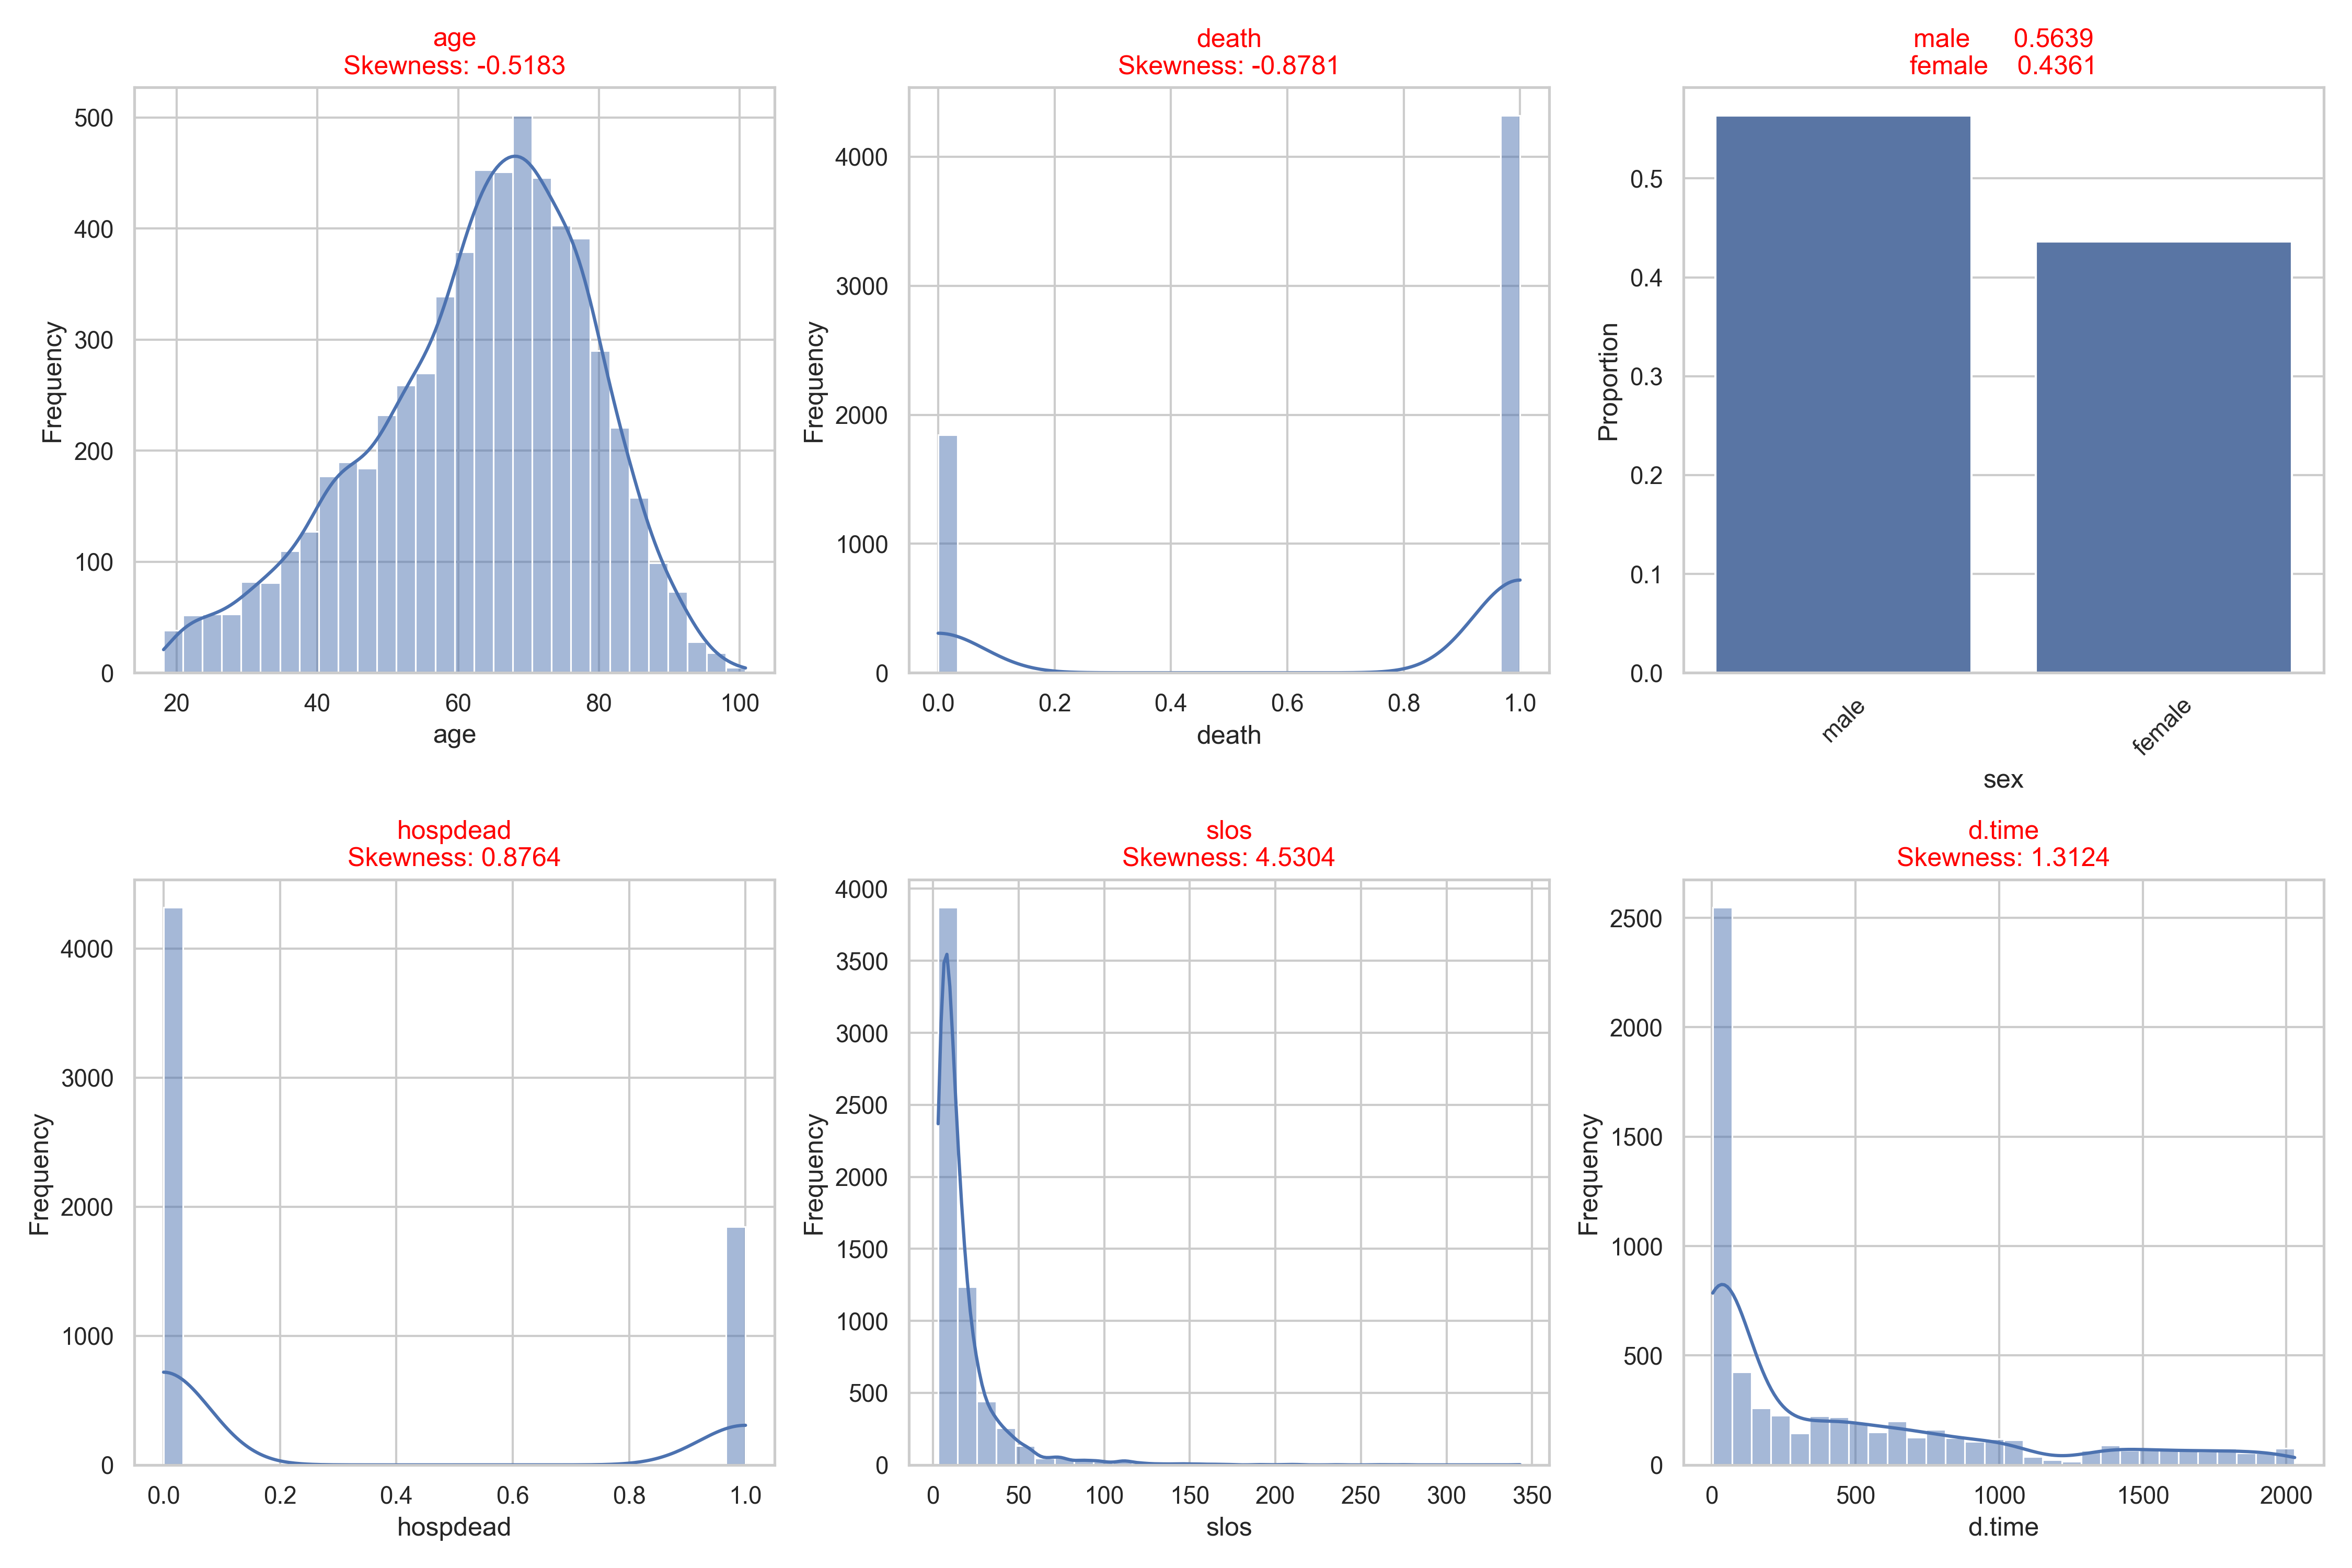
\includegraphics[width=0.8\textwidth]{../results/orginal_6th_feature_distributions.png}
    \caption{Descriptive statistics of the first 6 features SUPPORT2 dataset.}
    \label{fig:first_6_features}
\end{figure}

\begin{figure}[!h]
    \centering
    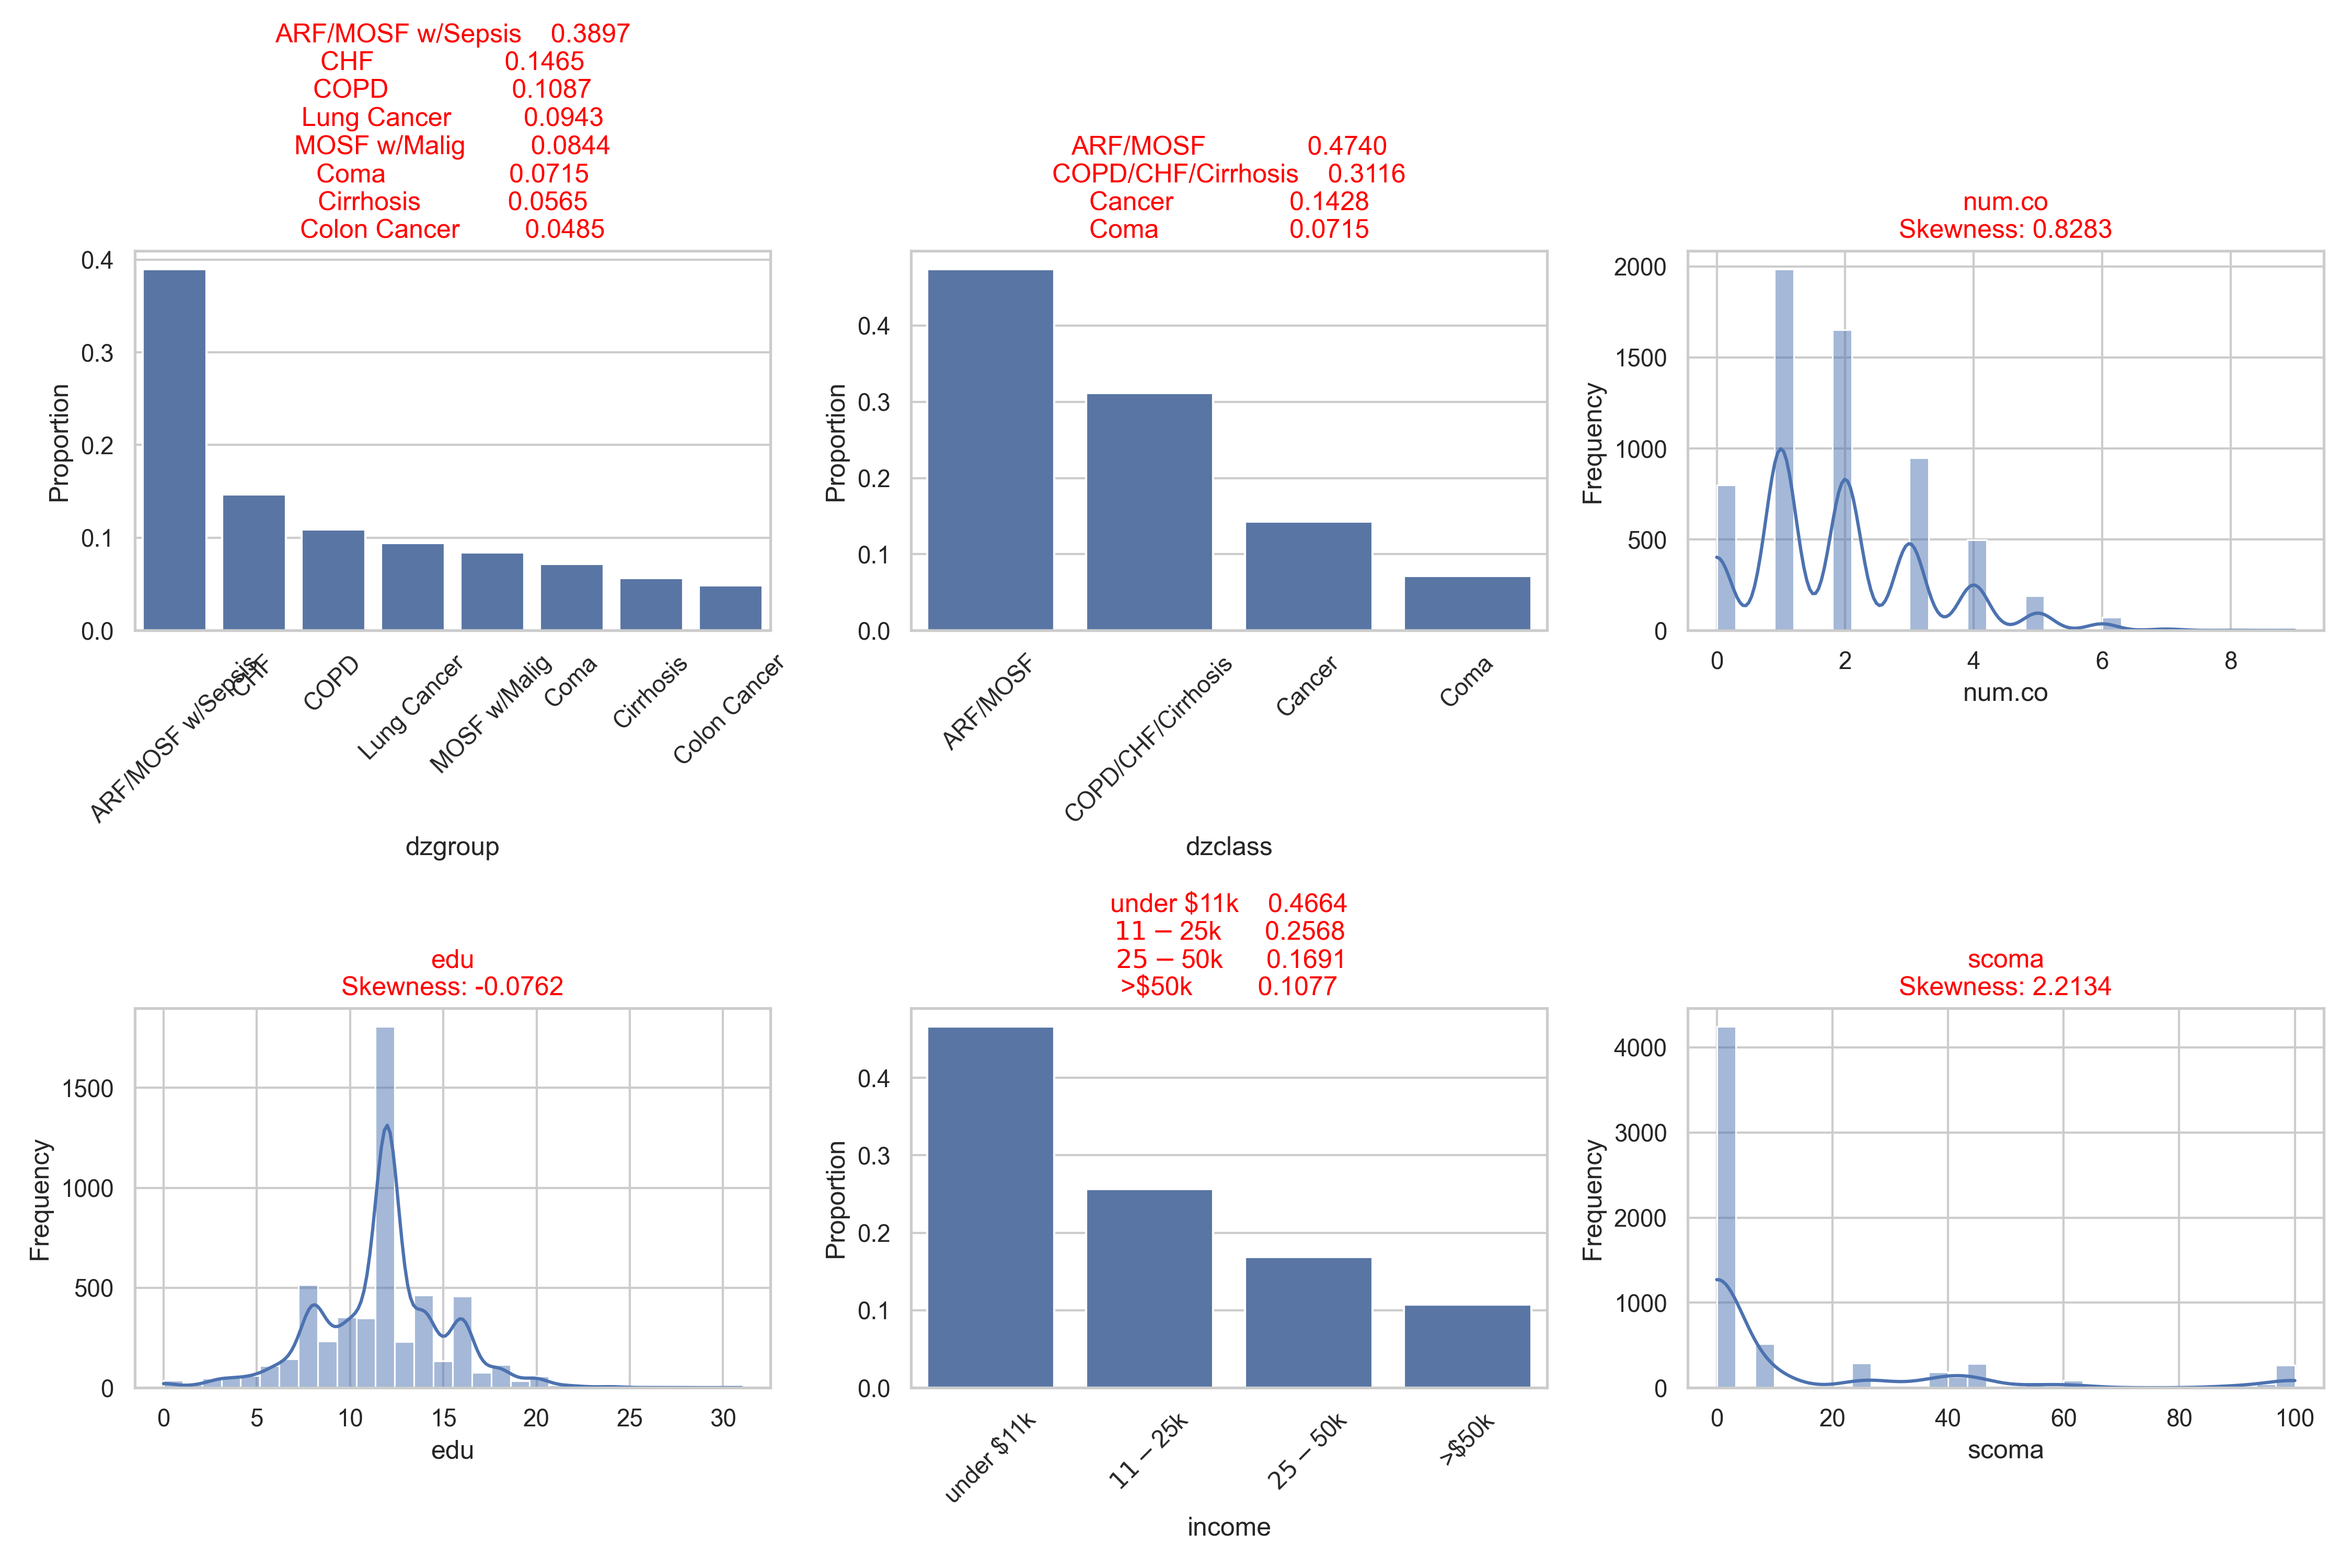
\includegraphics[width=0.8\textwidth]{../results/orginal_6_12th_feature_distributions.png}
    \caption{Descriptive statistics of the 7-12th features SUPPORT2 dataset.}
    \label{fig:7_12_features}
\end{figure}


\begin{figure}[!h]
    \centering
    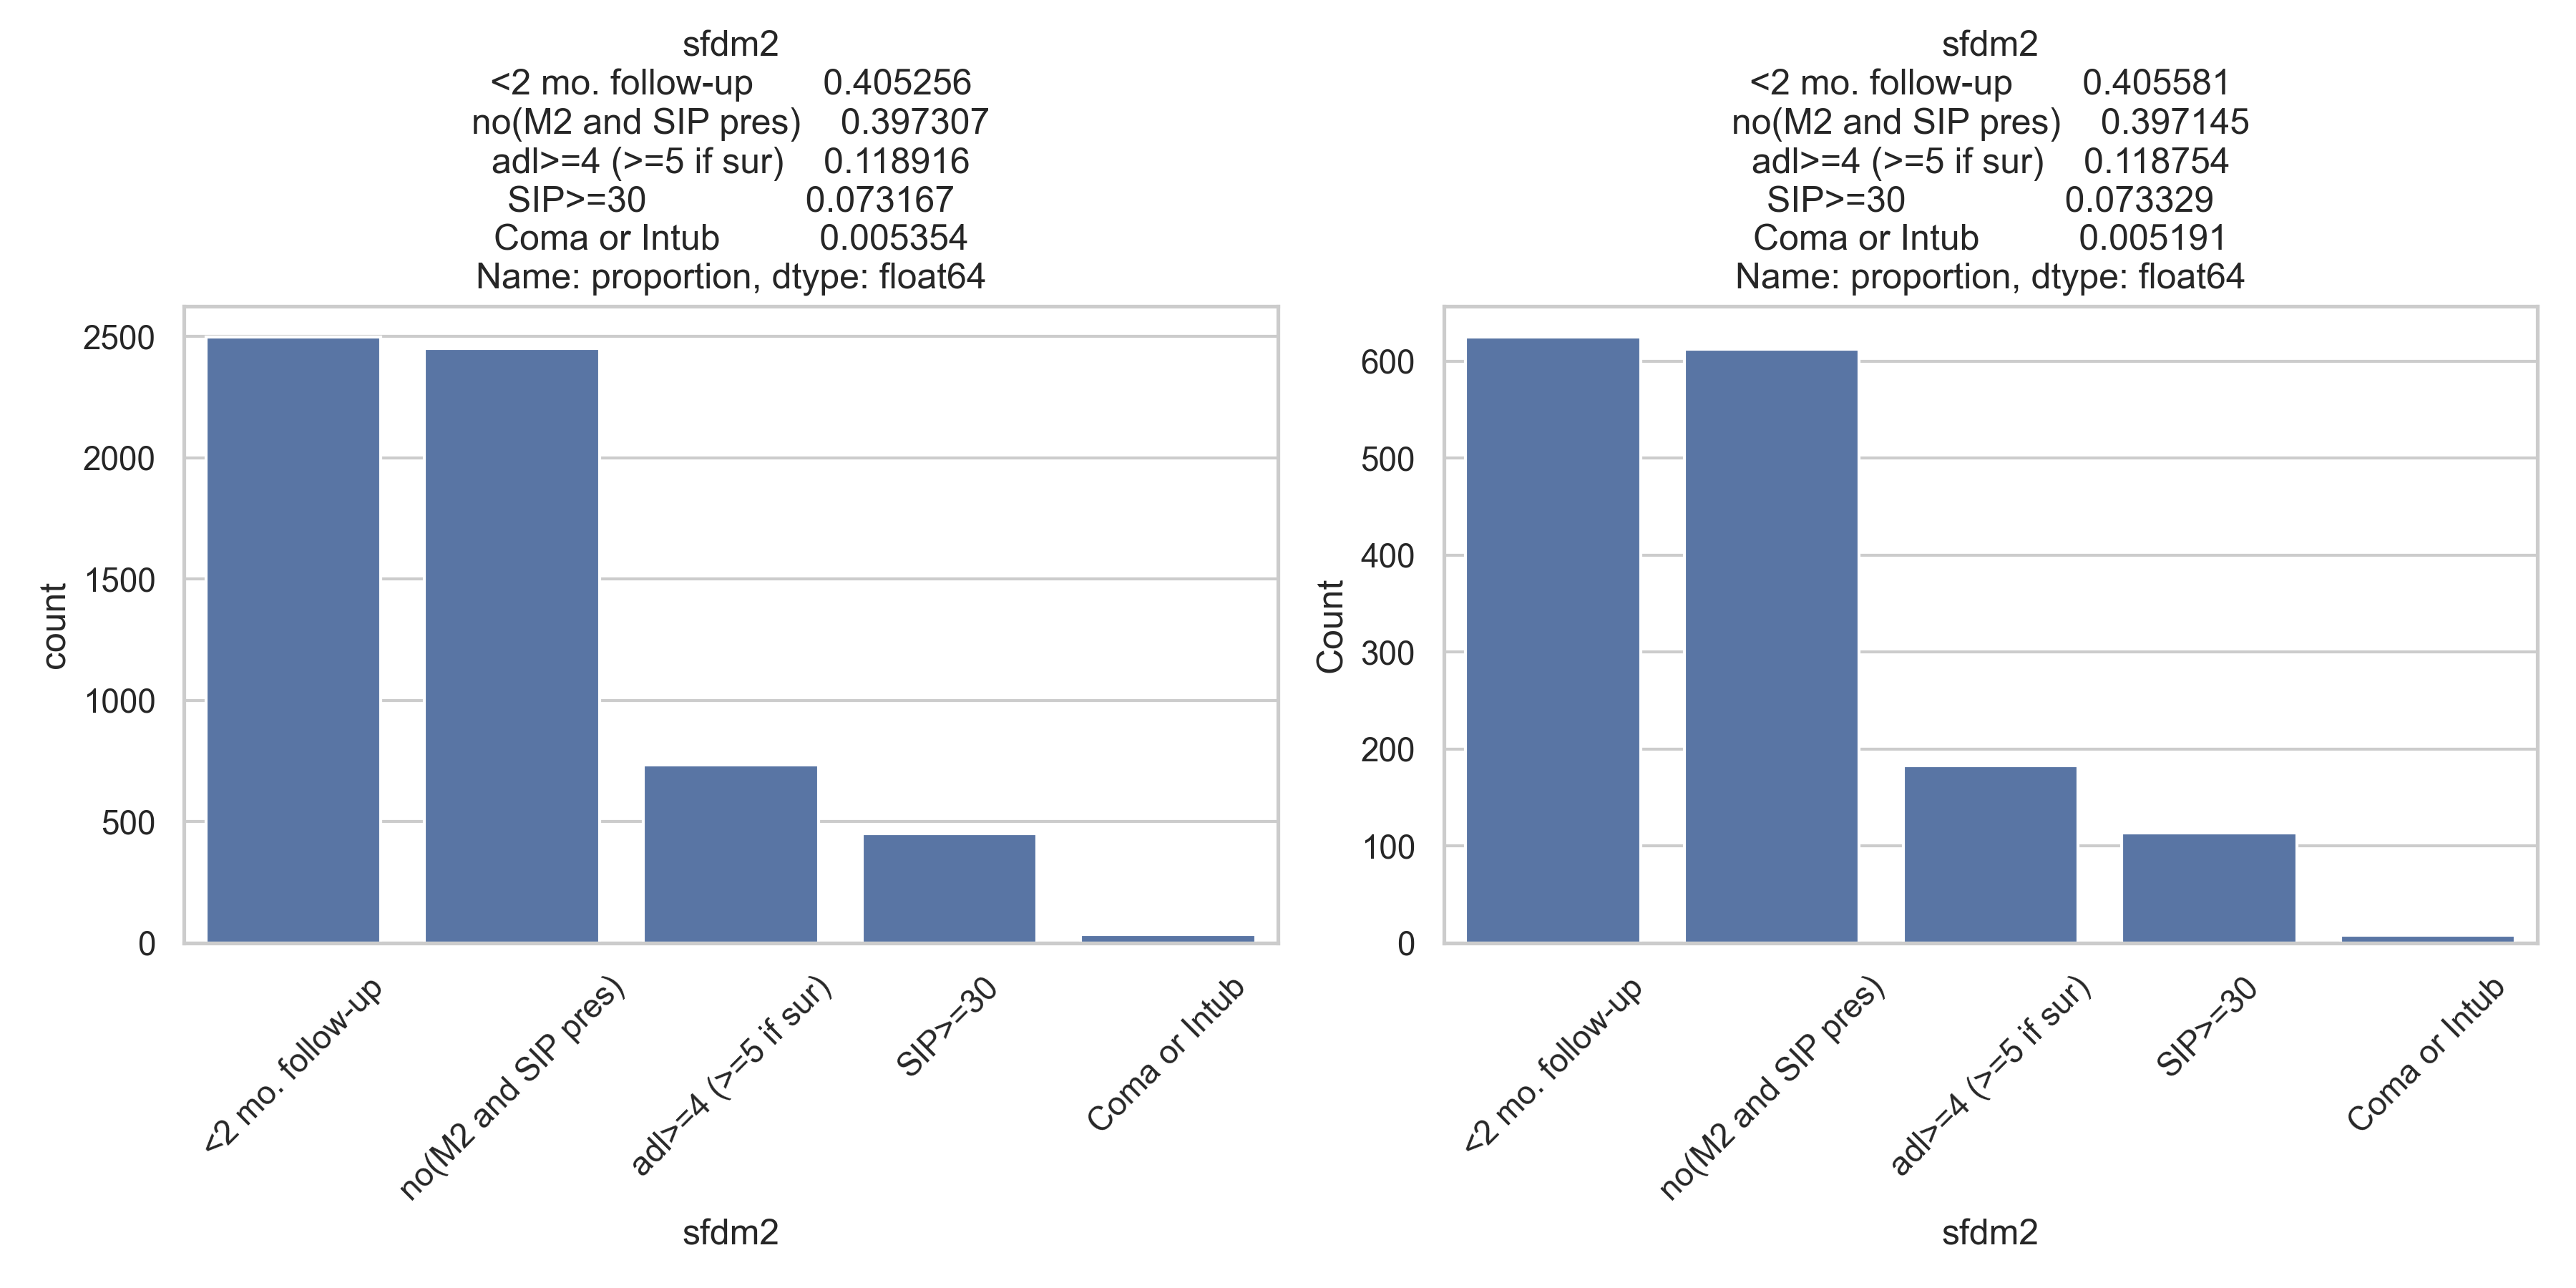
\includegraphics[width=0.8\textwidth]{../results/train_test_target_proportion.png}
    \caption{Distribution of the target variable SFDM2 in train(left) and test(right) data sets}
    \label{fig:train_test_target_proportion}
    \end{figure}

    

\end{document}